
\documentclass[a4paper,11pt]{exam}
\usepackage[T1]{fontenc}
\usepackage[utf8]{inputenc}
\usepackage{lmodern}
\usepackage[italian]{babel}
\usepackage{amsfonts}
\usepackage{amsmath}
\usepackage{amssymb}
\usepackage{fullpage}
\usepackage{graphicx}
\usepackage{wrapfig}
\usepackage{siunitx}
\usepackage{physics}
\usepackage{multicol}
\usepackage{geometry}
\usepackage{microtype}
\usepackage{siunitx}
\usepackage{physics}
\usepackage{multicol}

\newcommand{\um}[2]{\SI[output-decimal-marker={,}]{#1}{#2}}\usepackage{wrapfig}

\geometry{top=2cm, bottom=2cm, left=2cm, right=1.5cm}

\pagestyle{headandfoot}
\firstpageheadrule
\runningheadrule
\firstpageheader{VERIFICA DI PROVA}{ARGOMENTO A PIACERE}{1A}
\firstpagefooter{1 gennaio 2020}{TEMPO CONCESSO: 1H}{}
\runningfooter{1 gennaio 2020}{TEMPO CONCESSO: 1H}{}
\runningheader{VERIFICA DI PROVA}{ARGOMENTO A PIACERE}{1A}

\begin{document}

    

        \begin{center} 
        \fbox{\fbox{\parbox{17cm}{\centering Introduzione al quiz\\\ Modello n. 0                       
        }}}
        \end{center}
\begin{questions}

    
\question Il modulo del vettore $\vec{A}(3;4)$ è\\\
\begin{oneparchoices}
  \choice 8
  \choice 25
  \choice 5
  \choice 12
\end{oneparchoices}

    
\question Come si chiama il satellite naturale della Terra?\\\
\begin{oneparchoices}
  \choice ISS
  \choice Marte
  \choice Luna
  \choice Sole
\end{oneparchoices}

    
\question In che anno pare sia nato Gesù?\\\
\begin{oneparchoices}
  \choice 0
  \choice -80
  \choice 20
  \choice 2019
\end{oneparchoices}

    
\question Di che colore era il cavallo bianco di Napoleone?\\\
\begin{oneparchoices}
  \choice Bianco
  \choice Blu 
  \choice Marrone
  \choice Verde
\end{oneparchoices}

    
\question Se mischio blu e giallo che colore ottengo?\\\
\begin{oneparchoices}
  \choice Giallu
  \choice Blallo
  \choice Verde
  \choice Rosso
\end{oneparchoices}

    
\question Qual è la capitale d’Italia?\\\
\begin{oneparchoices}
  \choice Roma
  \choice Parigi
  \choice Milano
  \choice Berlino
\end{oneparchoices}

    
\question Dato il vettore $\vec{d}$ in figura, determina il modulo e la componente $d_x$: \begin{figure}[h!]   \begin{center}     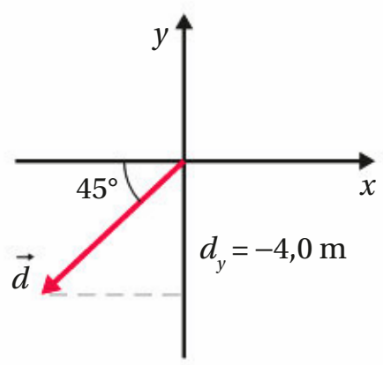
\includegraphics[scale=0.35]{vettored.png}   \end{center} \end{figure}\\\
\begin{oneparchoices}
  \choice -5,7 m; -4,0 m
  \choice 5,7 m; -4,0 m
  \choice -5,7 m; 4,0 m
  \choice 5,7 m; 4,0 m
\end{oneparchoices}

    
\question In quale anno il COVID ha fatto la sua comparsa?\\\
\begin{oneparchoices}
  \choice 1943
  \choice 2001
  \choice 2020
  \choice 2019
\end{oneparchoices}

    
\question Un gatto percorre 90,0~m verso sud e poi prosegue per altri 120~m verso ovest. Lo spostamento e la distanza percorsa sono rispettivamente\\\
\begin{oneparchoices}
  \choice 30~m e 210~m
  \choice 210~m e 150~m
  \choice 210~m e 210~m
  \choice 150~m e 210~m
\end{oneparchoices}

    
\question I due vettori $\vec{a}$ e $\vec{b}$ hanno lo stesso modulo e la stessa direzione. Quale delle seguenti affermazioni è falsa?\\\
\begin{oneparchoices}
  \choice La loro somma non può mai essere zero
  \choice I due vettori sono sicuramente uguali
  \choice Tutte le altre
  \choice La loro somma è sicuramente nulla
\end{oneparchoices}

    
\question Seguendo la mappa di un tesoro, un pirata cammina per 2,00~km verso nord-est, poi per 5,00~km verso est, quindi per 2,00~km verso sud-est e infine per 3,00~km verso ovest. Arrivato alla fine del percorso a che distanza si trova dalla posizione che occupava alla partenza?\\\
\begin{oneparchoices}
  \choice 4,59 km
  \choice 4,76 km
  \choice 6,32 km
  \choice 4,83 km
\end{oneparchoices}

    
\question Raddoppiando la distanza tra due cariche elettriche puntiformi, la forza elettrostatica diminuisce del\\\
\begin{oneparchoices}
  \choice 90\%
  \choice 75\%
  \choice 25\%
  \choice 50\%
\end{oneparchoices}

    
\end{questions}

    
    \newpage
    
    

        \begin{center} 
        \fbox{\fbox{\parbox{17cm}{\centering Introduzione al quiz\\\ Modello n. 1                       
        }}}
        \end{center}
\begin{questions}

    
\question Un gatto percorre 90,0~m verso sud e poi prosegue per altri 120~m verso ovest. Lo spostamento e la distanza percorsa sono rispettivamente\\\
\begin{oneparchoices}
  \choice 150~m e 210~m
  \choice 30~m e 210~m
  \choice 210~m e 150~m
  \choice 210~m e 210~m
\end{oneparchoices}

    
\question Qual è la capitale d’Italia?\\\
\begin{oneparchoices}
  \choice Roma
  \choice Milano
  \choice Parigi
  \choice Berlino
\end{oneparchoices}

    
\question Seguendo la mappa di un tesoro, un pirata cammina per 2,00~km verso nord-est, poi per 5,00~km verso est, quindi per 2,00~km verso sud-est e infine per 3,00~km verso ovest. Arrivato alla fine del percorso a che distanza si trova dalla posizione che occupava alla partenza?\\\
\begin{oneparchoices}
  \choice 4,59 km
  \choice 4,83 km
  \choice 4,76 km
  \choice 6,32 km
\end{oneparchoices}

    
\question Il modulo del vettore $\vec{A}(3;4)$ è\\\
\begin{oneparchoices}
  \choice 25
  \choice 5
  \choice 8
  \choice 12
\end{oneparchoices}

    
\question In che anno pare sia nato Gesù?\\\
\begin{oneparchoices}
  \choice 0
  \choice -80
  \choice 2019
  \choice 20
\end{oneparchoices}

    
\question Di che colore era il cavallo bianco di Napoleone?\\\
\begin{oneparchoices}
  \choice Marrone
  \choice Bianco
  \choice Verde
  \choice Blu 
\end{oneparchoices}

    
\question Raddoppiando la distanza tra due cariche elettriche puntiformi, la forza elettrostatica diminuisce del\\\
\begin{oneparchoices}
  \choice 90\%
  \choice 50\%
  \choice 25\%
  \choice 75\%
\end{oneparchoices}

    
\question In quale anno il COVID ha fatto la sua comparsa?\\\
\begin{oneparchoices}
  \choice 2019
  \choice 2001
  \choice 2020
  \choice 1943
\end{oneparchoices}

    
\question I due vettori $\vec{a}$ e $\vec{b}$ hanno lo stesso modulo e la stessa direzione. Quale delle seguenti affermazioni è falsa?\\\
\begin{oneparchoices}
  \choice La loro somma non può mai essere zero
  \choice I due vettori sono sicuramente uguali
  \choice Tutte le altre
  \choice La loro somma è sicuramente nulla
\end{oneparchoices}

    
\question Dato il vettore $\vec{d}$ in figura, determina il modulo e la componente $d_x$: \begin{figure}[h!]   \begin{center}     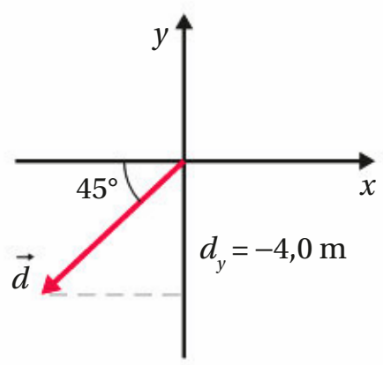
\includegraphics[scale=0.35]{vettored.png}   \end{center} \end{figure}\\\
\begin{oneparchoices}
  \choice 5,7 m; -4,0 m
  \choice 5,7 m; 4,0 m
  \choice -5,7 m; -4,0 m
  \choice -5,7 m; 4,0 m
\end{oneparchoices}

    
\question Se mischio blu e giallo che colore ottengo?\\\
\begin{oneparchoices}
  \choice Verde
  \choice Rosso
  \choice Blallo
  \choice Giallu
\end{oneparchoices}

    
\question Come si chiama il satellite naturale della Terra?\\\
\begin{oneparchoices}
  \choice Sole
  \choice Luna
  \choice Marte
  \choice ISS
\end{oneparchoices}

    
\end{questions}

    
    \newpage
    
    

        \begin{center} 
        \fbox{\fbox{\parbox{17cm}{\centering Introduzione al quiz\\\ Modello n. 2                       
        }}}
        \end{center}
\begin{questions}

    
\question Se mischio blu e giallo che colore ottengo?\\\
\begin{oneparchoices}
  \choice Blallo
  \choice Verde
  \choice Rosso
  \choice Giallu
\end{oneparchoices}

    
\question Dato il vettore $\vec{d}$ in figura, determina il modulo e la componente $d_x$: \begin{figure}[h!]   \begin{center}     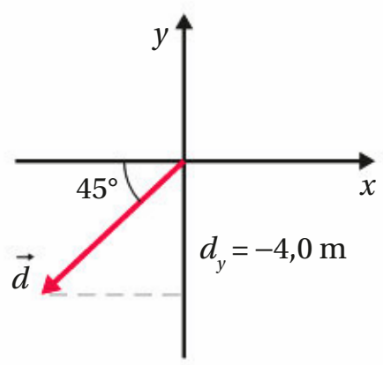
\includegraphics[scale=0.35]{vettored.png}   \end{center} \end{figure}\\\
\begin{oneparchoices}
  \choice -5,7 m; 4,0 m
  \choice 5,7 m; 4,0 m
  \choice 5,7 m; -4,0 m
  \choice -5,7 m; -4,0 m
\end{oneparchoices}

    
\question Il modulo del vettore $\vec{A}(3;4)$ è\\\
\begin{oneparchoices}
  \choice 8
  \choice 12
  \choice 5
  \choice 25
\end{oneparchoices}

    
\question In quale anno il COVID ha fatto la sua comparsa?\\\
\begin{oneparchoices}
  \choice 1943
  \choice 2019
  \choice 2001
  \choice 2020
\end{oneparchoices}

    
\question Come si chiama il satellite naturale della Terra?\\\
\begin{oneparchoices}
  \choice Luna
  \choice ISS
  \choice Marte
  \choice Sole
\end{oneparchoices}

    
\question Un gatto percorre 90,0~m verso sud e poi prosegue per altri 120~m verso ovest. Lo spostamento e la distanza percorsa sono rispettivamente\\\
\begin{oneparchoices}
  \choice 30~m e 210~m
  \choice 210~m e 150~m
  \choice 210~m e 210~m
  \choice 150~m e 210~m
\end{oneparchoices}

    
\question Raddoppiando la distanza tra due cariche elettriche puntiformi, la forza elettrostatica diminuisce del\\\
\begin{oneparchoices}
  \choice 25\%
  \choice 75\%
  \choice 90\%
  \choice 50\%
\end{oneparchoices}

    
\question In che anno pare sia nato Gesù?\\\
\begin{oneparchoices}
  \choice -80
  \choice 0
  \choice 20
  \choice 2019
\end{oneparchoices}

    
\question Qual è la capitale d’Italia?\\\
\begin{oneparchoices}
  \choice Berlino
  \choice Milano
  \choice Roma
  \choice Parigi
\end{oneparchoices}

    
\question Seguendo la mappa di un tesoro, un pirata cammina per 2,00~km verso nord-est, poi per 5,00~km verso est, quindi per 2,00~km verso sud-est e infine per 3,00~km verso ovest. Arrivato alla fine del percorso a che distanza si trova dalla posizione che occupava alla partenza?\\\
\begin{oneparchoices}
  \choice 6,32 km
  \choice 4,59 km
  \choice 4,76 km
  \choice 4,83 km
\end{oneparchoices}

    
\question Di che colore era il cavallo bianco di Napoleone?\\\
\begin{oneparchoices}
  \choice Bianco
  \choice Verde
  \choice Marrone
  \choice Blu 
\end{oneparchoices}

    
\question I due vettori $\vec{a}$ e $\vec{b}$ hanno lo stesso modulo e la stessa direzione. Quale delle seguenti affermazioni è falsa?\\\
\begin{oneparchoices}
  \choice Tutte le altre
  \choice I due vettori sono sicuramente uguali
  \choice La loro somma è sicuramente nulla
  \choice La loro somma non può mai essere zero
\end{oneparchoices}

    
\end{questions}

    
    \newpage
    
    

        \begin{center} 
        \fbox{\fbox{\parbox{17cm}{\centering Introduzione al quiz\\\ Modello n. 3                       
        }}}
        \end{center}
\begin{questions}

    
\question Il modulo del vettore $\vec{A}(3;4)$ è\\\
\begin{oneparchoices}
  \choice 12
  \choice 25
  \choice 8
  \choice 5
\end{oneparchoices}

    
\question Seguendo la mappa di un tesoro, un pirata cammina per 2,00~km verso nord-est, poi per 5,00~km verso est, quindi per 2,00~km verso sud-est e infine per 3,00~km verso ovest. Arrivato alla fine del percorso a che distanza si trova dalla posizione che occupava alla partenza?\\\
\begin{oneparchoices}
  \choice 6,32 km
  \choice 4,59 km
  \choice 4,76 km
  \choice 4,83 km
\end{oneparchoices}

    
\question I due vettori $\vec{a}$ e $\vec{b}$ hanno lo stesso modulo e la stessa direzione. Quale delle seguenti affermazioni è falsa?\\\
\begin{oneparchoices}
  \choice La loro somma non può mai essere zero
  \choice I due vettori sono sicuramente uguali
  \choice La loro somma è sicuramente nulla
  \choice Tutte le altre
\end{oneparchoices}

    
\question In quale anno il COVID ha fatto la sua comparsa?\\\
\begin{oneparchoices}
  \choice 2020
  \choice 2019
  \choice 2001
  \choice 1943
\end{oneparchoices}

    
\question Qual è la capitale d’Italia?\\\
\begin{oneparchoices}
  \choice Roma
  \choice Milano
  \choice Parigi
  \choice Berlino
\end{oneparchoices}

    
\question In che anno pare sia nato Gesù?\\\
\begin{oneparchoices}
  \choice 2019
  \choice 20
  \choice -80
  \choice 0
\end{oneparchoices}

    
\question Di che colore era il cavallo bianco di Napoleone?\\\
\begin{oneparchoices}
  \choice Blu 
  \choice Marrone
  \choice Bianco
  \choice Verde
\end{oneparchoices}

    
\question Raddoppiando la distanza tra due cariche elettriche puntiformi, la forza elettrostatica diminuisce del\\\
\begin{oneparchoices}
  \choice 50\%
  \choice 25\%
  \choice 90\%
  \choice 75\%
\end{oneparchoices}

    
\question Se mischio blu e giallo che colore ottengo?\\\
\begin{oneparchoices}
  \choice Verde
  \choice Blallo
  \choice Rosso
  \choice Giallu
\end{oneparchoices}

    
\question Un gatto percorre 90,0~m verso sud e poi prosegue per altri 120~m verso ovest. Lo spostamento e la distanza percorsa sono rispettivamente\\\
\begin{oneparchoices}
  \choice 30~m e 210~m
  \choice 210~m e 150~m
  \choice 150~m e 210~m
  \choice 210~m e 210~m
\end{oneparchoices}

    
\question Come si chiama il satellite naturale della Terra?\\\
\begin{oneparchoices}
  \choice Sole
  \choice Marte
  \choice Luna
  \choice ISS
\end{oneparchoices}

    
\question Dato il vettore $\vec{d}$ in figura, determina il modulo e la componente $d_x$: \begin{figure}[h!]   \begin{center}     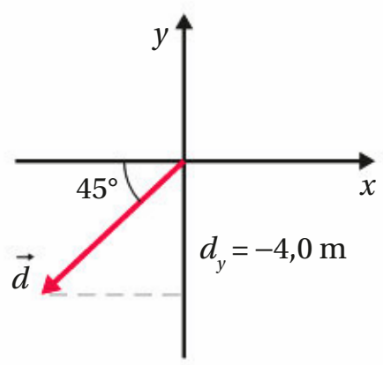
\includegraphics[scale=0.35]{vettored.png}   \end{center} \end{figure}\\\
\begin{oneparchoices}
  \choice 5,7 m; -4,0 m
  \choice -5,7 m; 4,0 m
  \choice 5,7 m; 4,0 m
  \choice -5,7 m; -4,0 m
\end{oneparchoices}

    
\end{questions}

    
    \newpage
    
    

        \begin{center} 
        \fbox{\fbox{\parbox{17cm}{\centering Introduzione al quiz\\\ Modello n. 4                       
        }}}
        \end{center}
\begin{questions}

    
\question In che anno pare sia nato Gesù?\\\
\begin{oneparchoices}
  \choice 2019
  \choice 20
  \choice -80
  \choice 0
\end{oneparchoices}

    
\question Qual è la capitale d’Italia?\\\
\begin{oneparchoices}
  \choice Roma
  \choice Milano
  \choice Parigi
  \choice Berlino
\end{oneparchoices}

    
\question Di che colore era il cavallo bianco di Napoleone?\\\
\begin{oneparchoices}
  \choice Marrone
  \choice Verde
  \choice Bianco
  \choice Blu 
\end{oneparchoices}

    
\question Il modulo del vettore $\vec{A}(3;4)$ è\\\
\begin{oneparchoices}
  \choice 8
  \choice 12
  \choice 25
  \choice 5
\end{oneparchoices}

    
\question Seguendo la mappa di un tesoro, un pirata cammina per 2,00~km verso nord-est, poi per 5,00~km verso est, quindi per 2,00~km verso sud-est e infine per 3,00~km verso ovest. Arrivato alla fine del percorso a che distanza si trova dalla posizione che occupava alla partenza?\\\
\begin{oneparchoices}
  \choice 4,59 km
  \choice 6,32 km
  \choice 4,83 km
  \choice 4,76 km
\end{oneparchoices}

    
\question I due vettori $\vec{a}$ e $\vec{b}$ hanno lo stesso modulo e la stessa direzione. Quale delle seguenti affermazioni è falsa?\\\
\begin{oneparchoices}
  \choice La loro somma è sicuramente nulla
  \choice La loro somma non può mai essere zero
  \choice I due vettori sono sicuramente uguali
  \choice Tutte le altre
\end{oneparchoices}

    
\question Dato il vettore $\vec{d}$ in figura, determina il modulo e la componente $d_x$: \begin{figure}[h!]   \begin{center}     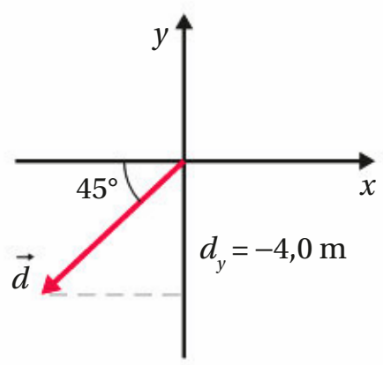
\includegraphics[scale=0.35]{vettored.png}   \end{center} \end{figure}\\\
\begin{oneparchoices}
  \choice 5,7 m; 4,0 m
  \choice -5,7 m; 4,0 m
  \choice 5,7 m; -4,0 m
  \choice -5,7 m; -4,0 m
\end{oneparchoices}

    
\question Un gatto percorre 90,0~m verso sud e poi prosegue per altri 120~m verso ovest. Lo spostamento e la distanza percorsa sono rispettivamente\\\
\begin{oneparchoices}
  \choice 150~m e 210~m
  \choice 210~m e 210~m
  \choice 30~m e 210~m
  \choice 210~m e 150~m
\end{oneparchoices}

    
\question In quale anno il COVID ha fatto la sua comparsa?\\\
\begin{oneparchoices}
  \choice 2001
  \choice 2020
  \choice 1943
  \choice 2019
\end{oneparchoices}

    
\question Raddoppiando la distanza tra due cariche elettriche puntiformi, la forza elettrostatica diminuisce del\\\
\begin{oneparchoices}
  \choice 75\%
  \choice 25\%
  \choice 90\%
  \choice 50\%
\end{oneparchoices}

    
\question Se mischio blu e giallo che colore ottengo?\\\
\begin{oneparchoices}
  \choice Giallu
  \choice Rosso
  \choice Blallo
  \choice Verde
\end{oneparchoices}

    
\question Come si chiama il satellite naturale della Terra?\\\
\begin{oneparchoices}
  \choice Luna
  \choice ISS
  \choice Marte
  \choice Sole
\end{oneparchoices}

    
\end{questions}

    
    \newpage
    
    

        \begin{center} 
        \fbox{\fbox{\parbox{17cm}{\centering Introduzione al quiz\\\ Modello n. 5                       
        }}}
        \end{center}
\begin{questions}

    
\question Un gatto percorre 90,0~m verso sud e poi prosegue per altri 120~m verso ovest. Lo spostamento e la distanza percorsa sono rispettivamente\\\
\begin{oneparchoices}
  \choice 30~m e 210~m
  \choice 210~m e 150~m
  \choice 210~m e 210~m
  \choice 150~m e 210~m
\end{oneparchoices}

    
\question I due vettori $\vec{a}$ e $\vec{b}$ hanno lo stesso modulo e la stessa direzione. Quale delle seguenti affermazioni è falsa?\\\
\begin{oneparchoices}
  \choice Tutte le altre
  \choice La loro somma non può mai essere zero
  \choice La loro somma è sicuramente nulla
  \choice I due vettori sono sicuramente uguali
\end{oneparchoices}

    
\question Se mischio blu e giallo che colore ottengo?\\\
\begin{oneparchoices}
  \choice Rosso
  \choice Giallu
  \choice Verde
  \choice Blallo
\end{oneparchoices}

    
\question Seguendo la mappa di un tesoro, un pirata cammina per 2,00~km verso nord-est, poi per 5,00~km verso est, quindi per 2,00~km verso sud-est e infine per 3,00~km verso ovest. Arrivato alla fine del percorso a che distanza si trova dalla posizione che occupava alla partenza?\\\
\begin{oneparchoices}
  \choice 6,32 km
  \choice 4,76 km
  \choice 4,59 km
  \choice 4,83 km
\end{oneparchoices}

    
\question In quale anno il COVID ha fatto la sua comparsa?\\\
\begin{oneparchoices}
  \choice 2001
  \choice 1943
  \choice 2020
  \choice 2019
\end{oneparchoices}

    
\question Come si chiama il satellite naturale della Terra?\\\
\begin{oneparchoices}
  \choice Sole
  \choice Marte
  \choice ISS
  \choice Luna
\end{oneparchoices}

    
\question Raddoppiando la distanza tra due cariche elettriche puntiformi, la forza elettrostatica diminuisce del\\\
\begin{oneparchoices}
  \choice 50\%
  \choice 25\%
  \choice 90\%
  \choice 75\%
\end{oneparchoices}

    
\question Di che colore era il cavallo bianco di Napoleone?\\\
\begin{oneparchoices}
  \choice Verde
  \choice Marrone
  \choice Bianco
  \choice Blu 
\end{oneparchoices}

    
\question Il modulo del vettore $\vec{A}(3;4)$ è\\\
\begin{oneparchoices}
  \choice 12
  \choice 25
  \choice 5
  \choice 8
\end{oneparchoices}

    
\question Dato il vettore $\vec{d}$ in figura, determina il modulo e la componente $d_x$: \begin{figure}[h!]   \begin{center}     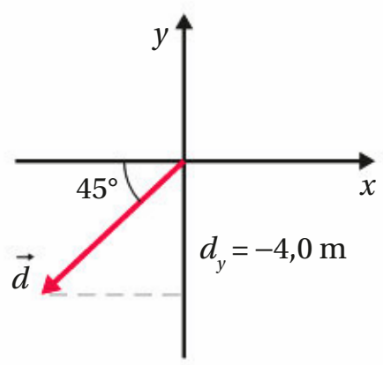
\includegraphics[scale=0.35]{vettored.png}   \end{center} \end{figure}\\\
\begin{oneparchoices}
  \choice -5,7 m; 4,0 m
  \choice 5,7 m; -4,0 m
  \choice 5,7 m; 4,0 m
  \choice -5,7 m; -4,0 m
\end{oneparchoices}

    
\question Qual è la capitale d’Italia?\\\
\begin{oneparchoices}
  \choice Roma
  \choice Berlino
  \choice Parigi
  \choice Milano
\end{oneparchoices}

    
\question In che anno pare sia nato Gesù?\\\
\begin{oneparchoices}
  \choice 20
  \choice -80
  \choice 2019
  \choice 0
\end{oneparchoices}

    
\end{questions}

    
    \newpage
    
    

        \begin{center} 
        \fbox{\fbox{\parbox{17cm}{\centering Introduzione al quiz\\\ Modello n. 6                       
        }}}
        \end{center}
\begin{questions}

    
\question Un gatto percorre 90,0~m verso sud e poi prosegue per altri 120~m verso ovest. Lo spostamento e la distanza percorsa sono rispettivamente\\\
\begin{oneparchoices}
  \choice 210~m e 150~m
  \choice 150~m e 210~m
  \choice 30~m e 210~m
  \choice 210~m e 210~m
\end{oneparchoices}

    
\question Il modulo del vettore $\vec{A}(3;4)$ è\\\
\begin{oneparchoices}
  \choice 25
  \choice 5
  \choice 12
  \choice 8
\end{oneparchoices}

    
\question I due vettori $\vec{a}$ e $\vec{b}$ hanno lo stesso modulo e la stessa direzione. Quale delle seguenti affermazioni è falsa?\\\
\begin{oneparchoices}
  \choice I due vettori sono sicuramente uguali
  \choice La loro somma non può mai essere zero
  \choice Tutte le altre
  \choice La loro somma è sicuramente nulla
\end{oneparchoices}

    
\question Se mischio blu e giallo che colore ottengo?\\\
\begin{oneparchoices}
  \choice Giallu
  \choice Blallo
  \choice Verde
  \choice Rosso
\end{oneparchoices}

    
\question In quale anno il COVID ha fatto la sua comparsa?\\\
\begin{oneparchoices}
  \choice 2020
  \choice 2001
  \choice 2019
  \choice 1943
\end{oneparchoices}

    
\question Come si chiama il satellite naturale della Terra?\\\
\begin{oneparchoices}
  \choice Marte
  \choice Sole
  \choice Luna
  \choice ISS
\end{oneparchoices}

    
\question Seguendo la mappa di un tesoro, un pirata cammina per 2,00~km verso nord-est, poi per 5,00~km verso est, quindi per 2,00~km verso sud-est e infine per 3,00~km verso ovest. Arrivato alla fine del percorso a che distanza si trova dalla posizione che occupava alla partenza?\\\
\begin{oneparchoices}
  \choice 4,59 km
  \choice 6,32 km
  \choice 4,76 km
  \choice 4,83 km
\end{oneparchoices}

    
\question Raddoppiando la distanza tra due cariche elettriche puntiformi, la forza elettrostatica diminuisce del\\\
\begin{oneparchoices}
  \choice 75\%
  \choice 25\%
  \choice 50\%
  \choice 90\%
\end{oneparchoices}

    
\question Di che colore era il cavallo bianco di Napoleone?\\\
\begin{oneparchoices}
  \choice Marrone
  \choice Blu 
  \choice Verde
  \choice Bianco
\end{oneparchoices}

    
\question In che anno pare sia nato Gesù?\\\
\begin{oneparchoices}
  \choice 2019
  \choice -80
  \choice 20
  \choice 0
\end{oneparchoices}

    
\question Qual è la capitale d’Italia?\\\
\begin{oneparchoices}
  \choice Berlino
  \choice Roma
  \choice Parigi
  \choice Milano
\end{oneparchoices}

    
\question Dato il vettore $\vec{d}$ in figura, determina il modulo e la componente $d_x$: \begin{figure}[h!]   \begin{center}     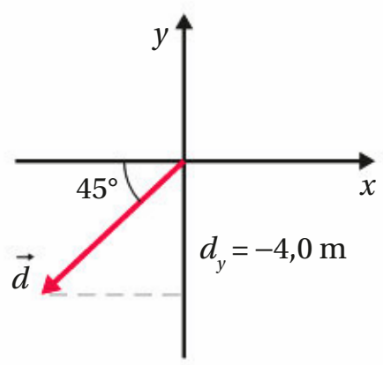
\includegraphics[scale=0.35]{vettored.png}   \end{center} \end{figure}\\\
\begin{oneparchoices}
  \choice 5,7 m; -4,0 m
  \choice -5,7 m; 4,0 m
  \choice 5,7 m; 4,0 m
  \choice -5,7 m; -4,0 m
\end{oneparchoices}

    
\end{questions}

    
    \newpage
    
    

        \begin{center} 
        \fbox{\fbox{\parbox{17cm}{\centering Introduzione al quiz\\\ Modello n. 7                       
        }}}
        \end{center}
\begin{questions}

    
\question Qual è la capitale d’Italia?\\\
\begin{oneparchoices}
  \choice Berlino
  \choice Parigi
  \choice Roma
  \choice Milano
\end{oneparchoices}

    
\question In quale anno il COVID ha fatto la sua comparsa?\\\
\begin{oneparchoices}
  \choice 2019
  \choice 1943
  \choice 2001
  \choice 2020
\end{oneparchoices}

    
\question Se mischio blu e giallo che colore ottengo?\\\
\begin{oneparchoices}
  \choice Blallo
  \choice Rosso
  \choice Verde
  \choice Giallu
\end{oneparchoices}

    
\question I due vettori $\vec{a}$ e $\vec{b}$ hanno lo stesso modulo e la stessa direzione. Quale delle seguenti affermazioni è falsa?\\\
\begin{oneparchoices}
  \choice La loro somma è sicuramente nulla
  \choice La loro somma non può mai essere zero
  \choice Tutte le altre
  \choice I due vettori sono sicuramente uguali
\end{oneparchoices}

    
\question Di che colore era il cavallo bianco di Napoleone?\\\
\begin{oneparchoices}
  \choice Verde
  \choice Blu 
  \choice Marrone
  \choice Bianco
\end{oneparchoices}

    
\question Dato il vettore $\vec{d}$ in figura, determina il modulo e la componente $d_x$: \begin{figure}[h!]   \begin{center}     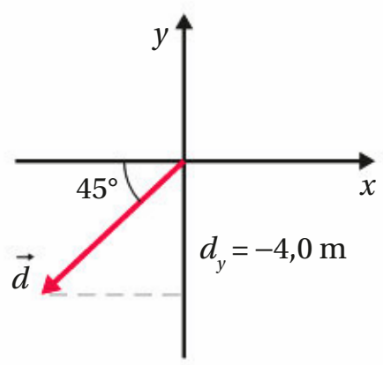
\includegraphics[scale=0.35]{vettored.png}   \end{center} \end{figure}\\\
\begin{oneparchoices}
  \choice 5,7 m; -4,0 m
  \choice -5,7 m; -4,0 m
  \choice -5,7 m; 4,0 m
  \choice 5,7 m; 4,0 m
\end{oneparchoices}

    
\question In che anno pare sia nato Gesù?\\\
\begin{oneparchoices}
  \choice 20
  \choice -80
  \choice 2019
  \choice 0
\end{oneparchoices}

    
\question Il modulo del vettore $\vec{A}(3;4)$ è\\\
\begin{oneparchoices}
  \choice 25
  \choice 12
  \choice 8
  \choice 5
\end{oneparchoices}

    
\question Seguendo la mappa di un tesoro, un pirata cammina per 2,00~km verso nord-est, poi per 5,00~km verso est, quindi per 2,00~km verso sud-est e infine per 3,00~km verso ovest. Arrivato alla fine del percorso a che distanza si trova dalla posizione che occupava alla partenza?\\\
\begin{oneparchoices}
  \choice 4,76 km
  \choice 6,32 km
  \choice 4,83 km
  \choice 4,59 km
\end{oneparchoices}

    
\question Raddoppiando la distanza tra due cariche elettriche puntiformi, la forza elettrostatica diminuisce del\\\
\begin{oneparchoices}
  \choice 25\%
  \choice 90\%
  \choice 75\%
  \choice 50\%
\end{oneparchoices}

    
\question Un gatto percorre 90,0~m verso sud e poi prosegue per altri 120~m verso ovest. Lo spostamento e la distanza percorsa sono rispettivamente\\\
\begin{oneparchoices}
  \choice 210~m e 210~m
  \choice 210~m e 150~m
  \choice 150~m e 210~m
  \choice 30~m e 210~m
\end{oneparchoices}

    
\question Come si chiama il satellite naturale della Terra?\\\
\begin{oneparchoices}
  \choice Luna
  \choice Marte
  \choice ISS
  \choice Sole
\end{oneparchoices}

    
\end{questions}

    
    \newpage
    
    

        \begin{center} 
        \fbox{\fbox{\parbox{17cm}{\centering Introduzione al quiz\\\ Modello n. 8                       
        }}}
        \end{center}
\begin{questions}

    
\question Di che colore era il cavallo bianco di Napoleone?\\\
\begin{oneparchoices}
  \choice Marrone
  \choice Bianco
  \choice Verde
  \choice Blu 
\end{oneparchoices}

    
\question Seguendo la mappa di un tesoro, un pirata cammina per 2,00~km verso nord-est, poi per 5,00~km verso est, quindi per 2,00~km verso sud-est e infine per 3,00~km verso ovest. Arrivato alla fine del percorso a che distanza si trova dalla posizione che occupava alla partenza?\\\
\begin{oneparchoices}
  \choice 4,83 km
  \choice 4,59 km
  \choice 6,32 km
  \choice 4,76 km
\end{oneparchoices}

    
\question Come si chiama il satellite naturale della Terra?\\\
\begin{oneparchoices}
  \choice ISS
  \choice Marte
  \choice Sole
  \choice Luna
\end{oneparchoices}

    
\question I due vettori $\vec{a}$ e $\vec{b}$ hanno lo stesso modulo e la stessa direzione. Quale delle seguenti affermazioni è falsa?\\\
\begin{oneparchoices}
  \choice Tutte le altre
  \choice La loro somma è sicuramente nulla
  \choice La loro somma non può mai essere zero
  \choice I due vettori sono sicuramente uguali
\end{oneparchoices}

    
\question In quale anno il COVID ha fatto la sua comparsa?\\\
\begin{oneparchoices}
  \choice 2020
  \choice 2001
  \choice 2019
  \choice 1943
\end{oneparchoices}

    
\question Qual è la capitale d’Italia?\\\
\begin{oneparchoices}
  \choice Milano
  \choice Roma
  \choice Berlino
  \choice Parigi
\end{oneparchoices}

    
\question In che anno pare sia nato Gesù?\\\
\begin{oneparchoices}
  \choice 20
  \choice 2019
  \choice -80
  \choice 0
\end{oneparchoices}

    
\question Raddoppiando la distanza tra due cariche elettriche puntiformi, la forza elettrostatica diminuisce del\\\
\begin{oneparchoices}
  \choice 75\%
  \choice 90\%
  \choice 25\%
  \choice 50\%
\end{oneparchoices}

    
\question Un gatto percorre 90,0~m verso sud e poi prosegue per altri 120~m verso ovest. Lo spostamento e la distanza percorsa sono rispettivamente\\\
\begin{oneparchoices}
  \choice 210~m e 150~m
  \choice 150~m e 210~m
  \choice 30~m e 210~m
  \choice 210~m e 210~m
\end{oneparchoices}

    
\question Il modulo del vettore $\vec{A}(3;4)$ è\\\
\begin{oneparchoices}
  \choice 12
  \choice 25
  \choice 5
  \choice 8
\end{oneparchoices}

    
\question Dato il vettore $\vec{d}$ in figura, determina il modulo e la componente $d_x$: \begin{figure}[h!]   \begin{center}     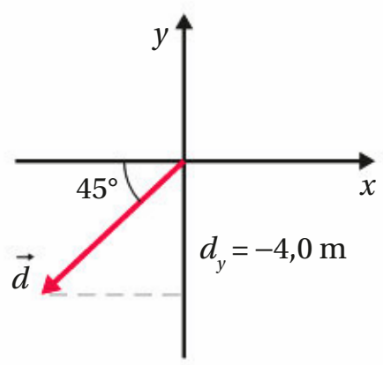
\includegraphics[scale=0.35]{vettored.png}   \end{center} \end{figure}\\\
\begin{oneparchoices}
  \choice 5,7 m; 4,0 m
  \choice 5,7 m; -4,0 m
  \choice -5,7 m; 4,0 m
  \choice -5,7 m; -4,0 m
\end{oneparchoices}

    
\question Se mischio blu e giallo che colore ottengo?\\\
\begin{oneparchoices}
  \choice Giallu
  \choice Blallo
  \choice Verde
  \choice Rosso
\end{oneparchoices}

    
\end{questions}

    
    \newpage
    
    

        \begin{center} 
        \fbox{\fbox{\parbox{17cm}{\centering Introduzione al quiz\\\ Modello n. 9                       
        }}}
        \end{center}
\begin{questions}

    
\question Di che colore era il cavallo bianco di Napoleone?\\\
\begin{oneparchoices}
  \choice Marrone
  \choice Bianco
  \choice Blu 
  \choice Verde
\end{oneparchoices}

    
\question Dato il vettore $\vec{d}$ in figura, determina il modulo e la componente $d_x$: \begin{figure}[h!]   \begin{center}     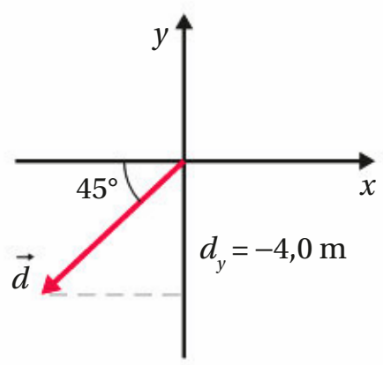
\includegraphics[scale=0.35]{vettored.png}   \end{center} \end{figure}\\\
\begin{oneparchoices}
  \choice 5,7 m; -4,0 m
  \choice -5,7 m; 4,0 m
  \choice 5,7 m; 4,0 m
  \choice -5,7 m; -4,0 m
\end{oneparchoices}

    
\question In che anno pare sia nato Gesù?\\\
\begin{oneparchoices}
  \choice 2019
  \choice 0
  \choice -80
  \choice 20
\end{oneparchoices}

    
\question Un gatto percorre 90,0~m verso sud e poi prosegue per altri 120~m verso ovest. Lo spostamento e la distanza percorsa sono rispettivamente\\\
\begin{oneparchoices}
  \choice 30~m e 210~m
  \choice 210~m e 210~m
  \choice 150~m e 210~m
  \choice 210~m e 150~m
\end{oneparchoices}

    
\question Raddoppiando la distanza tra due cariche elettriche puntiformi, la forza elettrostatica diminuisce del\\\
\begin{oneparchoices}
  \choice 25\%
  \choice 90\%
  \choice 75\%
  \choice 50\%
\end{oneparchoices}

    
\question Qual è la capitale d’Italia?\\\
\begin{oneparchoices}
  \choice Berlino
  \choice Roma
  \choice Milano
  \choice Parigi
\end{oneparchoices}

    
\question Il modulo del vettore $\vec{A}(3;4)$ è\\\
\begin{oneparchoices}
  \choice 25
  \choice 8
  \choice 5
  \choice 12
\end{oneparchoices}

    
\question I due vettori $\vec{a}$ e $\vec{b}$ hanno lo stesso modulo e la stessa direzione. Quale delle seguenti affermazioni è falsa?\\\
\begin{oneparchoices}
  \choice La loro somma non può mai essere zero
  \choice Tutte le altre
  \choice I due vettori sono sicuramente uguali
  \choice La loro somma è sicuramente nulla
\end{oneparchoices}

    
\question Come si chiama il satellite naturale della Terra?\\\
\begin{oneparchoices}
  \choice Luna
  \choice ISS
  \choice Marte
  \choice Sole
\end{oneparchoices}

    
\question Seguendo la mappa di un tesoro, un pirata cammina per 2,00~km verso nord-est, poi per 5,00~km verso est, quindi per 2,00~km verso sud-est e infine per 3,00~km verso ovest. Arrivato alla fine del percorso a che distanza si trova dalla posizione che occupava alla partenza?\\\
\begin{oneparchoices}
  \choice 6,32 km
  \choice 4,76 km
  \choice 4,83 km
  \choice 4,59 km
\end{oneparchoices}

    
\question In quale anno il COVID ha fatto la sua comparsa?\\\
\begin{oneparchoices}
  \choice 2020
  \choice 2019
  \choice 2001
  \choice 1943
\end{oneparchoices}

    
\question Se mischio blu e giallo che colore ottengo?\\\
\begin{oneparchoices}
  \choice Giallu
  \choice Rosso
  \choice Blallo
  \choice Verde
\end{oneparchoices}

    
\end{questions}

    
    \newpage
    
    

        \begin{center} 
        \fbox{\fbox{\parbox{17cm}{\centering Introduzione al quiz\\\ Modello n. 10                       
        }}}
        \end{center}
\begin{questions}

    
\question In quale anno il COVID ha fatto la sua comparsa?\\\
\begin{oneparchoices}
  \choice 2019
  \choice 1943
  \choice 2001
  \choice 2020
\end{oneparchoices}

    
\question Qual è la capitale d’Italia?\\\
\begin{oneparchoices}
  \choice Milano
  \choice Berlino
  \choice Parigi
  \choice Roma
\end{oneparchoices}

    
\question Raddoppiando la distanza tra due cariche elettriche puntiformi, la forza elettrostatica diminuisce del\\\
\begin{oneparchoices}
  \choice 90\%
  \choice 25\%
  \choice 75\%
  \choice 50\%
\end{oneparchoices}

    
\question Il modulo del vettore $\vec{A}(3;4)$ è\\\
\begin{oneparchoices}
  \choice 8
  \choice 5
  \choice 12
  \choice 25
\end{oneparchoices}

    
\question Dato il vettore $\vec{d}$ in figura, determina il modulo e la componente $d_x$: \begin{figure}[h!]   \begin{center}     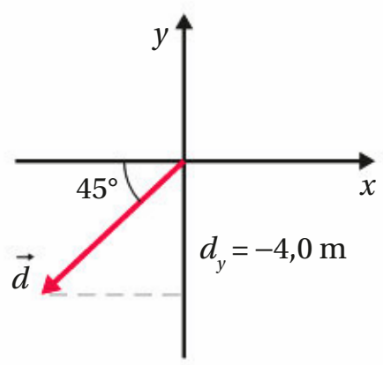
\includegraphics[scale=0.35]{vettored.png}   \end{center} \end{figure}\\\
\begin{oneparchoices}
  \choice 5,7 m; 4,0 m
  \choice -5,7 m; -4,0 m
  \choice -5,7 m; 4,0 m
  \choice 5,7 m; -4,0 m
\end{oneparchoices}

    
\question I due vettori $\vec{a}$ e $\vec{b}$ hanno lo stesso modulo e la stessa direzione. Quale delle seguenti affermazioni è falsa?\\\
\begin{oneparchoices}
  \choice Tutte le altre
  \choice La loro somma non può mai essere zero
  \choice La loro somma è sicuramente nulla
  \choice I due vettori sono sicuramente uguali
\end{oneparchoices}

    
\question Di che colore era il cavallo bianco di Napoleone?\\\
\begin{oneparchoices}
  \choice Verde
  \choice Marrone
  \choice Bianco
  \choice Blu 
\end{oneparchoices}

    
\question Come si chiama il satellite naturale della Terra?\\\
\begin{oneparchoices}
  \choice Sole
  \choice ISS
  \choice Marte
  \choice Luna
\end{oneparchoices}

    
\question Se mischio blu e giallo che colore ottengo?\\\
\begin{oneparchoices}
  \choice Giallu
  \choice Verde
  \choice Blallo
  \choice Rosso
\end{oneparchoices}

    
\question In che anno pare sia nato Gesù?\\\
\begin{oneparchoices}
  \choice -80
  \choice 2019
  \choice 0
  \choice 20
\end{oneparchoices}

    
\question Seguendo la mappa di un tesoro, un pirata cammina per 2,00~km verso nord-est, poi per 5,00~km verso est, quindi per 2,00~km verso sud-est e infine per 3,00~km verso ovest. Arrivato alla fine del percorso a che distanza si trova dalla posizione che occupava alla partenza?\\\
\begin{oneparchoices}
  \choice 6,32 km
  \choice 4,76 km
  \choice 4,83 km
  \choice 4,59 km
\end{oneparchoices}

    
\question Un gatto percorre 90,0~m verso sud e poi prosegue per altri 120~m verso ovest. Lo spostamento e la distanza percorsa sono rispettivamente\\\
\begin{oneparchoices}
  \choice 210~m e 150~m
  \choice 150~m e 210~m
  \choice 210~m e 210~m
  \choice 30~m e 210~m
\end{oneparchoices}

    
\end{questions}

    
    \newpage
    
    

        \begin{center} 
        \fbox{\fbox{\parbox{17cm}{\centering Introduzione al quiz\\\ Modello n. 11                       
        }}}
        \end{center}
\begin{questions}

    
\question Qual è la capitale d’Italia?\\\
\begin{oneparchoices}
  \choice Parigi
  \choice Berlino
  \choice Milano
  \choice Roma
\end{oneparchoices}

    
\question In quale anno il COVID ha fatto la sua comparsa?\\\
\begin{oneparchoices}
  \choice 2019
  \choice 2001
  \choice 1943
  \choice 2020
\end{oneparchoices}

    
\question Come si chiama il satellite naturale della Terra?\\\
\begin{oneparchoices}
  \choice Sole
  \choice Marte
  \choice ISS
  \choice Luna
\end{oneparchoices}

    
\question In che anno pare sia nato Gesù?\\\
\begin{oneparchoices}
  \choice 2019
  \choice 0
  \choice -80
  \choice 20
\end{oneparchoices}

    
\question Dato il vettore $\vec{d}$ in figura, determina il modulo e la componente $d_x$: \begin{figure}[h!]   \begin{center}     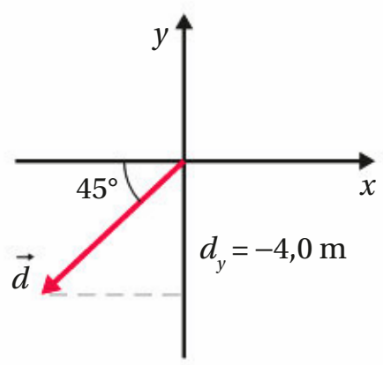
\includegraphics[scale=0.35]{vettored.png}   \end{center} \end{figure}\\\
\begin{oneparchoices}
  \choice -5,7 m; 4,0 m
  \choice -5,7 m; -4,0 m
  \choice 5,7 m; 4,0 m
  \choice 5,7 m; -4,0 m
\end{oneparchoices}

    
\question Di che colore era il cavallo bianco di Napoleone?\\\
\begin{oneparchoices}
  \choice Blu 
  \choice Verde
  \choice Bianco
  \choice Marrone
\end{oneparchoices}

    
\question Il modulo del vettore $\vec{A}(3;4)$ è\\\
\begin{oneparchoices}
  \choice 25
  \choice 12
  \choice 8
  \choice 5
\end{oneparchoices}

    
\question Un gatto percorre 90,0~m verso sud e poi prosegue per altri 120~m verso ovest. Lo spostamento e la distanza percorsa sono rispettivamente\\\
\begin{oneparchoices}
  \choice 150~m e 210~m
  \choice 30~m e 210~m
  \choice 210~m e 150~m
  \choice 210~m e 210~m
\end{oneparchoices}

    
\question Se mischio blu e giallo che colore ottengo?\\\
\begin{oneparchoices}
  \choice Rosso
  \choice Giallu
  \choice Blallo
  \choice Verde
\end{oneparchoices}

    
\question Seguendo la mappa di un tesoro, un pirata cammina per 2,00~km verso nord-est, poi per 5,00~km verso est, quindi per 2,00~km verso sud-est e infine per 3,00~km verso ovest. Arrivato alla fine del percorso a che distanza si trova dalla posizione che occupava alla partenza?\\\
\begin{oneparchoices}
  \choice 4,83 km
  \choice 6,32 km
  \choice 4,76 km
  \choice 4,59 km
\end{oneparchoices}

    
\question I due vettori $\vec{a}$ e $\vec{b}$ hanno lo stesso modulo e la stessa direzione. Quale delle seguenti affermazioni è falsa?\\\
\begin{oneparchoices}
  \choice La loro somma non può mai essere zero
  \choice Tutte le altre
  \choice I due vettori sono sicuramente uguali
  \choice La loro somma è sicuramente nulla
\end{oneparchoices}

    
\question Raddoppiando la distanza tra due cariche elettriche puntiformi, la forza elettrostatica diminuisce del\\\
\begin{oneparchoices}
  \choice 75\%
  \choice 25\%
  \choice 50\%
  \choice 90\%
\end{oneparchoices}

    
\end{questions}

    
    \newpage
    
    

        \begin{center} 
        \fbox{\fbox{\parbox{17cm}{\centering Introduzione al quiz\\\ Modello n. 12                       
        }}}
        \end{center}
\begin{questions}

    
\question Il modulo del vettore $\vec{A}(3;4)$ è\\\
\begin{oneparchoices}
  \choice 25
  \choice 8
  \choice 12
  \choice 5
\end{oneparchoices}

    
\question In che anno pare sia nato Gesù?\\\
\begin{oneparchoices}
  \choice 2019
  \choice -80
  \choice 0
  \choice 20
\end{oneparchoices}

    
\question Se mischio blu e giallo che colore ottengo?\\\
\begin{oneparchoices}
  \choice Blallo
  \choice Giallu
  \choice Rosso
  \choice Verde
\end{oneparchoices}

    
\question Raddoppiando la distanza tra due cariche elettriche puntiformi, la forza elettrostatica diminuisce del\\\
\begin{oneparchoices}
  \choice 25\%
  \choice 50\%
  \choice 90\%
  \choice 75\%
\end{oneparchoices}

    
\question Seguendo la mappa di un tesoro, un pirata cammina per 2,00~km verso nord-est, poi per 5,00~km verso est, quindi per 2,00~km verso sud-est e infine per 3,00~km verso ovest. Arrivato alla fine del percorso a che distanza si trova dalla posizione che occupava alla partenza?\\\
\begin{oneparchoices}
  \choice 4,59 km
  \choice 4,76 km
  \choice 4,83 km
  \choice 6,32 km
\end{oneparchoices}

    
\question Dato il vettore $\vec{d}$ in figura, determina il modulo e la componente $d_x$: \begin{figure}[h!]   \begin{center}     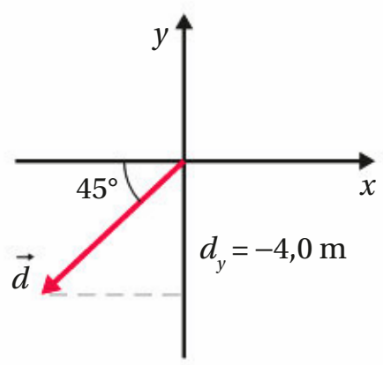
\includegraphics[scale=0.35]{vettored.png}   \end{center} \end{figure}\\\
\begin{oneparchoices}
  \choice 5,7 m; 4,0 m
  \choice 5,7 m; -4,0 m
  \choice -5,7 m; 4,0 m
  \choice -5,7 m; -4,0 m
\end{oneparchoices}

    
\question I due vettori $\vec{a}$ e $\vec{b}$ hanno lo stesso modulo e la stessa direzione. Quale delle seguenti affermazioni è falsa?\\\
\begin{oneparchoices}
  \choice La loro somma non può mai essere zero
  \choice I due vettori sono sicuramente uguali
  \choice Tutte le altre
  \choice La loro somma è sicuramente nulla
\end{oneparchoices}

    
\question Un gatto percorre 90,0~m verso sud e poi prosegue per altri 120~m verso ovest. Lo spostamento e la distanza percorsa sono rispettivamente\\\
\begin{oneparchoices}
  \choice 210~m e 210~m
  \choice 150~m e 210~m
  \choice 30~m e 210~m
  \choice 210~m e 150~m
\end{oneparchoices}

    
\question Qual è la capitale d’Italia?\\\
\begin{oneparchoices}
  \choice Milano
  \choice Roma
  \choice Parigi
  \choice Berlino
\end{oneparchoices}

    
\question Come si chiama il satellite naturale della Terra?\\\
\begin{oneparchoices}
  \choice Sole
  \choice Luna
  \choice Marte
  \choice ISS
\end{oneparchoices}

    
\question In quale anno il COVID ha fatto la sua comparsa?\\\
\begin{oneparchoices}
  \choice 2020
  \choice 2019
  \choice 2001
  \choice 1943
\end{oneparchoices}

    
\question Di che colore era il cavallo bianco di Napoleone?\\\
\begin{oneparchoices}
  \choice Verde
  \choice Bianco
  \choice Marrone
  \choice Blu 
\end{oneparchoices}

    
\end{questions}

    
    \newpage
    
    

        \begin{center} 
        \fbox{\fbox{\parbox{17cm}{\centering Introduzione al quiz\\\ Modello n. 13                       
        }}}
        \end{center}
\begin{questions}

    
\question Se mischio blu e giallo che colore ottengo?\\\
\begin{oneparchoices}
  \choice Giallu
  \choice Verde
  \choice Blallo
  \choice Rosso
\end{oneparchoices}

    
\question Di che colore era il cavallo bianco di Napoleone?\\\
\begin{oneparchoices}
  \choice Marrone
  \choice Verde
  \choice Blu 
  \choice Bianco
\end{oneparchoices}

    
\question Raddoppiando la distanza tra due cariche elettriche puntiformi, la forza elettrostatica diminuisce del\\\
\begin{oneparchoices}
  \choice 90\%
  \choice 25\%
  \choice 50\%
  \choice 75\%
\end{oneparchoices}

    
\question Qual è la capitale d’Italia?\\\
\begin{oneparchoices}
  \choice Parigi
  \choice Berlino
  \choice Roma
  \choice Milano
\end{oneparchoices}

    
\question Un gatto percorre 90,0~m verso sud e poi prosegue per altri 120~m verso ovest. Lo spostamento e la distanza percorsa sono rispettivamente\\\
\begin{oneparchoices}
  \choice 210~m e 150~m
  \choice 150~m e 210~m
  \choice 210~m e 210~m
  \choice 30~m e 210~m
\end{oneparchoices}

    
\question Come si chiama il satellite naturale della Terra?\\\
\begin{oneparchoices}
  \choice Sole
  \choice Luna
  \choice ISS
  \choice Marte
\end{oneparchoices}

    
\question Seguendo la mappa di un tesoro, un pirata cammina per 2,00~km verso nord-est, poi per 5,00~km verso est, quindi per 2,00~km verso sud-est e infine per 3,00~km verso ovest. Arrivato alla fine del percorso a che distanza si trova dalla posizione che occupava alla partenza?\\\
\begin{oneparchoices}
  \choice 4,59 km
  \choice 6,32 km
  \choice 4,76 km
  \choice 4,83 km
\end{oneparchoices}

    
\question In che anno pare sia nato Gesù?\\\
\begin{oneparchoices}
  \choice -80
  \choice 2019
  \choice 20
  \choice 0
\end{oneparchoices}

    
\question Il modulo del vettore $\vec{A}(3;4)$ è\\\
\begin{oneparchoices}
  \choice 8
  \choice 5
  \choice 12
  \choice 25
\end{oneparchoices}

    
\question I due vettori $\vec{a}$ e $\vec{b}$ hanno lo stesso modulo e la stessa direzione. Quale delle seguenti affermazioni è falsa?\\\
\begin{oneparchoices}
  \choice Tutte le altre
  \choice I due vettori sono sicuramente uguali
  \choice La loro somma è sicuramente nulla
  \choice La loro somma non può mai essere zero
\end{oneparchoices}

    
\question Dato il vettore $\vec{d}$ in figura, determina il modulo e la componente $d_x$: \begin{figure}[h!]   \begin{center}     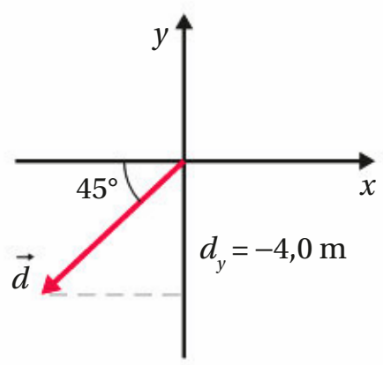
\includegraphics[scale=0.35]{vettored.png}   \end{center} \end{figure}\\\
\begin{oneparchoices}
  \choice 5,7 m; 4,0 m
  \choice 5,7 m; -4,0 m
  \choice -5,7 m; 4,0 m
  \choice -5,7 m; -4,0 m
\end{oneparchoices}

    
\question In quale anno il COVID ha fatto la sua comparsa?\\\
\begin{oneparchoices}
  \choice 2019
  \choice 2020
  \choice 1943
  \choice 2001
\end{oneparchoices}

    
\end{questions}

    
    \newpage
    
    

        \begin{center} 
        \fbox{\fbox{\parbox{17cm}{\centering Introduzione al quiz\\\ Modello n. 14                       
        }}}
        \end{center}
\begin{questions}

    
\question Se mischio blu e giallo che colore ottengo?\\\
\begin{oneparchoices}
  \choice Verde
  \choice Blallo
  \choice Rosso
  \choice Giallu
\end{oneparchoices}

    
\question I due vettori $\vec{a}$ e $\vec{b}$ hanno lo stesso modulo e la stessa direzione. Quale delle seguenti affermazioni è falsa?\\\
\begin{oneparchoices}
  \choice La loro somma non può mai essere zero
  \choice Tutte le altre
  \choice La loro somma è sicuramente nulla
  \choice I due vettori sono sicuramente uguali
\end{oneparchoices}

    
\question Come si chiama il satellite naturale della Terra?\\\
\begin{oneparchoices}
  \choice Marte
  \choice ISS
  \choice Sole
  \choice Luna
\end{oneparchoices}

    
\question Raddoppiando la distanza tra due cariche elettriche puntiformi, la forza elettrostatica diminuisce del\\\
\begin{oneparchoices}
  \choice 50\%
  \choice 90\%
  \choice 75\%
  \choice 25\%
\end{oneparchoices}

    
\question Il modulo del vettore $\vec{A}(3;4)$ è\\\
\begin{oneparchoices}
  \choice 12
  \choice 5
  \choice 8
  \choice 25
\end{oneparchoices}

    
\question Di che colore era il cavallo bianco di Napoleone?\\\
\begin{oneparchoices}
  \choice Verde
  \choice Bianco
  \choice Blu 
  \choice Marrone
\end{oneparchoices}

    
\question In che anno pare sia nato Gesù?\\\
\begin{oneparchoices}
  \choice 2019
  \choice 0
  \choice 20
  \choice -80
\end{oneparchoices}

    
\question Un gatto percorre 90,0~m verso sud e poi prosegue per altri 120~m verso ovest. Lo spostamento e la distanza percorsa sono rispettivamente\\\
\begin{oneparchoices}
  \choice 30~m e 210~m
  \choice 210~m e 150~m
  \choice 210~m e 210~m
  \choice 150~m e 210~m
\end{oneparchoices}

    
\question Dato il vettore $\vec{d}$ in figura, determina il modulo e la componente $d_x$: \begin{figure}[h!]   \begin{center}     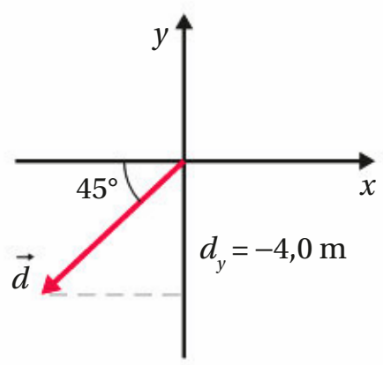
\includegraphics[scale=0.35]{vettored.png}   \end{center} \end{figure}\\\
\begin{oneparchoices}
  \choice 5,7 m; 4,0 m
  \choice 5,7 m; -4,0 m
  \choice -5,7 m; 4,0 m
  \choice -5,7 m; -4,0 m
\end{oneparchoices}

    
\question Seguendo la mappa di un tesoro, un pirata cammina per 2,00~km verso nord-est, poi per 5,00~km verso est, quindi per 2,00~km verso sud-est e infine per 3,00~km verso ovest. Arrivato alla fine del percorso a che distanza si trova dalla posizione che occupava alla partenza?\\\
\begin{oneparchoices}
  \choice 4,59 km
  \choice 4,83 km
  \choice 4,76 km
  \choice 6,32 km
\end{oneparchoices}

    
\question Qual è la capitale d’Italia?\\\
\begin{oneparchoices}
  \choice Parigi
  \choice Roma
  \choice Milano
  \choice Berlino
\end{oneparchoices}

    
\question In quale anno il COVID ha fatto la sua comparsa?\\\
\begin{oneparchoices}
  \choice 2020
  \choice 2019
  \choice 1943
  \choice 2001
\end{oneparchoices}

    
\end{questions}

    
    \newpage
    
    

        \begin{center} 
        \fbox{\fbox{\parbox{17cm}{\centering Introduzione al quiz\\\ Modello n. 15                       
        }}}
        \end{center}
\begin{questions}

    
\question In che anno pare sia nato Gesù?\\\
\begin{oneparchoices}
  \choice 0
  \choice 2019
  \choice -80
  \choice 20
\end{oneparchoices}

    
\question Raddoppiando la distanza tra due cariche elettriche puntiformi, la forza elettrostatica diminuisce del\\\
\begin{oneparchoices}
  \choice 90\%
  \choice 25\%
  \choice 50\%
  \choice 75\%
\end{oneparchoices}

    
\question Un gatto percorre 90,0~m verso sud e poi prosegue per altri 120~m verso ovest. Lo spostamento e la distanza percorsa sono rispettivamente\\\
\begin{oneparchoices}
  \choice 210~m e 150~m
  \choice 150~m e 210~m
  \choice 210~m e 210~m
  \choice 30~m e 210~m
\end{oneparchoices}

    
\question Seguendo la mappa di un tesoro, un pirata cammina per 2,00~km verso nord-est, poi per 5,00~km verso est, quindi per 2,00~km verso sud-est e infine per 3,00~km verso ovest. Arrivato alla fine del percorso a che distanza si trova dalla posizione che occupava alla partenza?\\\
\begin{oneparchoices}
  \choice 6,32 km
  \choice 4,76 km
  \choice 4,83 km
  \choice 4,59 km
\end{oneparchoices}

    
\question Dato il vettore $\vec{d}$ in figura, determina il modulo e la componente $d_x$: \begin{figure}[h!]   \begin{center}     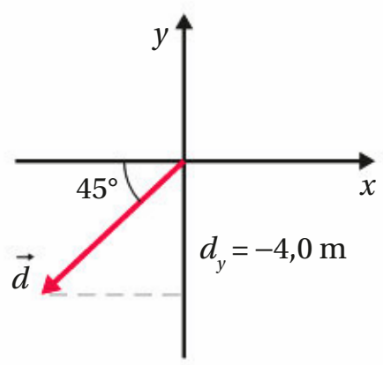
\includegraphics[scale=0.35]{vettored.png}   \end{center} \end{figure}\\\
\begin{oneparchoices}
  \choice -5,7 m; 4,0 m
  \choice -5,7 m; -4,0 m
  \choice 5,7 m; -4,0 m
  \choice 5,7 m; 4,0 m
\end{oneparchoices}

    
\question In quale anno il COVID ha fatto la sua comparsa?\\\
\begin{oneparchoices}
  \choice 1943
  \choice 2001
  \choice 2020
  \choice 2019
\end{oneparchoices}

    
\question Di che colore era il cavallo bianco di Napoleone?\\\
\begin{oneparchoices}
  \choice Verde
  \choice Bianco
  \choice Blu 
  \choice Marrone
\end{oneparchoices}

    
\question Se mischio blu e giallo che colore ottengo?\\\
\begin{oneparchoices}
  \choice Giallu
  \choice Verde
  \choice Blallo
  \choice Rosso
\end{oneparchoices}

    
\question Qual è la capitale d’Italia?\\\
\begin{oneparchoices}
  \choice Roma
  \choice Berlino
  \choice Parigi
  \choice Milano
\end{oneparchoices}

    
\question I due vettori $\vec{a}$ e $\vec{b}$ hanno lo stesso modulo e la stessa direzione. Quale delle seguenti affermazioni è falsa?\\\
\begin{oneparchoices}
  \choice La loro somma è sicuramente nulla
  \choice La loro somma non può mai essere zero
  \choice I due vettori sono sicuramente uguali
  \choice Tutte le altre
\end{oneparchoices}

    
\question Il modulo del vettore $\vec{A}(3;4)$ è\\\
\begin{oneparchoices}
  \choice 12
  \choice 25
  \choice 8
  \choice 5
\end{oneparchoices}

    
\question Come si chiama il satellite naturale della Terra?\\\
\begin{oneparchoices}
  \choice Marte
  \choice Sole
  \choice ISS
  \choice Luna
\end{oneparchoices}

    
\end{questions}

    
    \newpage
    
    

        \begin{center} 
        \fbox{\fbox{\parbox{17cm}{\centering Introduzione al quiz\\\ Modello n. 16                       
        }}}
        \end{center}
\begin{questions}

    
\question Un gatto percorre 90,0~m verso sud e poi prosegue per altri 120~m verso ovest. Lo spostamento e la distanza percorsa sono rispettivamente\\\
\begin{oneparchoices}
  \choice 30~m e 210~m
  \choice 210~m e 150~m
  \choice 150~m e 210~m
  \choice 210~m e 210~m
\end{oneparchoices}

    
\question In che anno pare sia nato Gesù?\\\
\begin{oneparchoices}
  \choice -80
  \choice 20
  \choice 2019
  \choice 0
\end{oneparchoices}

    
\question Dato il vettore $\vec{d}$ in figura, determina il modulo e la componente $d_x$: \begin{figure}[h!]   \begin{center}     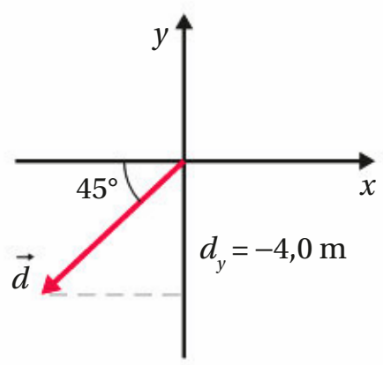
\includegraphics[scale=0.35]{vettored.png}   \end{center} \end{figure}\\\
\begin{oneparchoices}
  \choice -5,7 m; 4,0 m
  \choice 5,7 m; -4,0 m
  \choice 5,7 m; 4,0 m
  \choice -5,7 m; -4,0 m
\end{oneparchoices}

    
\question Il modulo del vettore $\vec{A}(3;4)$ è\\\
\begin{oneparchoices}
  \choice 25
  \choice 8
  \choice 5
  \choice 12
\end{oneparchoices}

    
\question In quale anno il COVID ha fatto la sua comparsa?\\\
\begin{oneparchoices}
  \choice 2001
  \choice 2020
  \choice 2019
  \choice 1943
\end{oneparchoices}

    
\question Qual è la capitale d’Italia?\\\
\begin{oneparchoices}
  \choice Berlino
  \choice Parigi
  \choice Milano
  \choice Roma
\end{oneparchoices}

    
\question Se mischio blu e giallo che colore ottengo?\\\
\begin{oneparchoices}
  \choice Verde
  \choice Blallo
  \choice Rosso
  \choice Giallu
\end{oneparchoices}

    
\question I due vettori $\vec{a}$ e $\vec{b}$ hanno lo stesso modulo e la stessa direzione. Quale delle seguenti affermazioni è falsa?\\\
\begin{oneparchoices}
  \choice La loro somma è sicuramente nulla
  \choice I due vettori sono sicuramente uguali
  \choice Tutte le altre
  \choice La loro somma non può mai essere zero
\end{oneparchoices}

    
\question Come si chiama il satellite naturale della Terra?\\\
\begin{oneparchoices}
  \choice Marte
  \choice Sole
  \choice Luna
  \choice ISS
\end{oneparchoices}

    
\question Raddoppiando la distanza tra due cariche elettriche puntiformi, la forza elettrostatica diminuisce del\\\
\begin{oneparchoices}
  \choice 75\%
  \choice 25\%
  \choice 50\%
  \choice 90\%
\end{oneparchoices}

    
\question Di che colore era il cavallo bianco di Napoleone?\\\
\begin{oneparchoices}
  \choice Bianco
  \choice Verde
  \choice Blu 
  \choice Marrone
\end{oneparchoices}

    
\question Seguendo la mappa di un tesoro, un pirata cammina per 2,00~km verso nord-est, poi per 5,00~km verso est, quindi per 2,00~km verso sud-est e infine per 3,00~km verso ovest. Arrivato alla fine del percorso a che distanza si trova dalla posizione che occupava alla partenza?\\\
\begin{oneparchoices}
  \choice 4,76 km
  \choice 4,83 km
  \choice 6,32 km
  \choice 4,59 km
\end{oneparchoices}

    
\end{questions}

    
    \newpage
    
    

        \begin{center} 
        \fbox{\fbox{\parbox{17cm}{\centering Introduzione al quiz\\\ Modello n. 17                       
        }}}
        \end{center}
\begin{questions}

    
\question Qual è la capitale d’Italia?\\\
\begin{oneparchoices}
  \choice Roma
  \choice Parigi
  \choice Berlino
  \choice Milano
\end{oneparchoices}

    
\question Il modulo del vettore $\vec{A}(3;4)$ è\\\
\begin{oneparchoices}
  \choice 12
  \choice 8
  \choice 25
  \choice 5
\end{oneparchoices}

    
\question Raddoppiando la distanza tra due cariche elettriche puntiformi, la forza elettrostatica diminuisce del\\\
\begin{oneparchoices}
  \choice 25\%
  \choice 90\%
  \choice 75\%
  \choice 50\%
\end{oneparchoices}

    
\question Seguendo la mappa di un tesoro, un pirata cammina per 2,00~km verso nord-est, poi per 5,00~km verso est, quindi per 2,00~km verso sud-est e infine per 3,00~km verso ovest. Arrivato alla fine del percorso a che distanza si trova dalla posizione che occupava alla partenza?\\\
\begin{oneparchoices}
  \choice 6,32 km
  \choice 4,76 km
  \choice 4,59 km
  \choice 4,83 km
\end{oneparchoices}

    
\question Se mischio blu e giallo che colore ottengo?\\\
\begin{oneparchoices}
  \choice Rosso
  \choice Verde
  \choice Giallu
  \choice Blallo
\end{oneparchoices}

    
\question In che anno pare sia nato Gesù?\\\
\begin{oneparchoices}
  \choice 0
  \choice 20
  \choice 2019
  \choice -80
\end{oneparchoices}

    
\question In quale anno il COVID ha fatto la sua comparsa?\\\
\begin{oneparchoices}
  \choice 2001
  \choice 1943
  \choice 2020
  \choice 2019
\end{oneparchoices}

    
\question I due vettori $\vec{a}$ e $\vec{b}$ hanno lo stesso modulo e la stessa direzione. Quale delle seguenti affermazioni è falsa?\\\
\begin{oneparchoices}
  \choice La loro somma non può mai essere zero
  \choice I due vettori sono sicuramente uguali
  \choice Tutte le altre
  \choice La loro somma è sicuramente nulla
\end{oneparchoices}

    
\question Di che colore era il cavallo bianco di Napoleone?\\\
\begin{oneparchoices}
  \choice Marrone
  \choice Verde
  \choice Bianco
  \choice Blu 
\end{oneparchoices}

    
\question Dato il vettore $\vec{d}$ in figura, determina il modulo e la componente $d_x$: \begin{figure}[h!]   \begin{center}     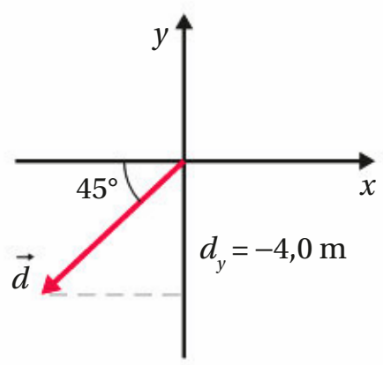
\includegraphics[scale=0.35]{vettored.png}   \end{center} \end{figure}\\\
\begin{oneparchoices}
  \choice 5,7 m; -4,0 m
  \choice -5,7 m; 4,0 m
  \choice -5,7 m; -4,0 m
  \choice 5,7 m; 4,0 m
\end{oneparchoices}

    
\question Un gatto percorre 90,0~m verso sud e poi prosegue per altri 120~m verso ovest. Lo spostamento e la distanza percorsa sono rispettivamente\\\
\begin{oneparchoices}
  \choice 210~m e 210~m
  \choice 150~m e 210~m
  \choice 210~m e 150~m
  \choice 30~m e 210~m
\end{oneparchoices}

    
\question Come si chiama il satellite naturale della Terra?\\\
\begin{oneparchoices}
  \choice Luna
  \choice Sole
  \choice Marte
  \choice ISS
\end{oneparchoices}

    
\end{questions}

    
    \newpage
    
    

        \begin{center} 
        \fbox{\fbox{\parbox{17cm}{\centering Introduzione al quiz\\\ Modello n. 18                       
        }}}
        \end{center}
\begin{questions}

    
\question In quale anno il COVID ha fatto la sua comparsa?\\\
\begin{oneparchoices}
  \choice 2019
  \choice 2001
  \choice 1943
  \choice 2020
\end{oneparchoices}

    
\question Se mischio blu e giallo che colore ottengo?\\\
\begin{oneparchoices}
  \choice Rosso
  \choice Blallo
  \choice Giallu
  \choice Verde
\end{oneparchoices}

    
\question Raddoppiando la distanza tra due cariche elettriche puntiformi, la forza elettrostatica diminuisce del\\\
\begin{oneparchoices}
  \choice 90\%
  \choice 25\%
  \choice 50\%
  \choice 75\%
\end{oneparchoices}

    
\question In che anno pare sia nato Gesù?\\\
\begin{oneparchoices}
  \choice 2019
  \choice 0
  \choice -80
  \choice 20
\end{oneparchoices}

    
\question I due vettori $\vec{a}$ e $\vec{b}$ hanno lo stesso modulo e la stessa direzione. Quale delle seguenti affermazioni è falsa?\\\
\begin{oneparchoices}
  \choice La loro somma non può mai essere zero
  \choice Tutte le altre
  \choice La loro somma è sicuramente nulla
  \choice I due vettori sono sicuramente uguali
\end{oneparchoices}

    
\question Il modulo del vettore $\vec{A}(3;4)$ è\\\
\begin{oneparchoices}
  \choice 25
  \choice 5
  \choice 8
  \choice 12
\end{oneparchoices}

    
\question Di che colore era il cavallo bianco di Napoleone?\\\
\begin{oneparchoices}
  \choice Verde
  \choice Blu 
  \choice Marrone
  \choice Bianco
\end{oneparchoices}

    
\question Un gatto percorre 90,0~m verso sud e poi prosegue per altri 120~m verso ovest. Lo spostamento e la distanza percorsa sono rispettivamente\\\
\begin{oneparchoices}
  \choice 30~m e 210~m
  \choice 210~m e 210~m
  \choice 150~m e 210~m
  \choice 210~m e 150~m
\end{oneparchoices}

    
\question Dato il vettore $\vec{d}$ in figura, determina il modulo e la componente $d_x$: \begin{figure}[h!]   \begin{center}     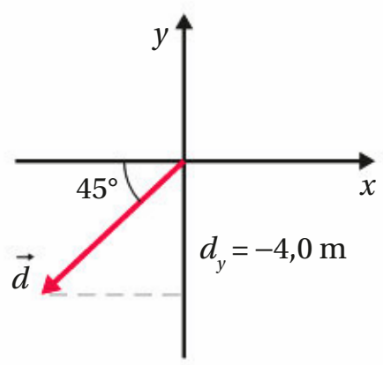
\includegraphics[scale=0.35]{vettored.png}   \end{center} \end{figure}\\\
\begin{oneparchoices}
  \choice -5,7 m; -4,0 m
  \choice 5,7 m; -4,0 m
  \choice -5,7 m; 4,0 m
  \choice 5,7 m; 4,0 m
\end{oneparchoices}

    
\question Qual è la capitale d’Italia?\\\
\begin{oneparchoices}
  \choice Berlino
  \choice Parigi
  \choice Milano
  \choice Roma
\end{oneparchoices}

    
\question Come si chiama il satellite naturale della Terra?\\\
\begin{oneparchoices}
  \choice Marte
  \choice ISS
  \choice Luna
  \choice Sole
\end{oneparchoices}

    
\question Seguendo la mappa di un tesoro, un pirata cammina per 2,00~km verso nord-est, poi per 5,00~km verso est, quindi per 2,00~km verso sud-est e infine per 3,00~km verso ovest. Arrivato alla fine del percorso a che distanza si trova dalla posizione che occupava alla partenza?\\\
\begin{oneparchoices}
  \choice 4,76 km
  \choice 4,59 km
  \choice 4,83 km
  \choice 6,32 km
\end{oneparchoices}

    
\end{questions}

    
    \newpage
    
    

        \begin{center} 
        \fbox{\fbox{\parbox{17cm}{\centering Introduzione al quiz\\\ Modello n. 19                       
        }}}
        \end{center}
\begin{questions}

    
\question Raddoppiando la distanza tra due cariche elettriche puntiformi, la forza elettrostatica diminuisce del\\\
\begin{oneparchoices}
  \choice 25\%
  \choice 75\%
  \choice 90\%
  \choice 50\%
\end{oneparchoices}

    
\question In che anno pare sia nato Gesù?\\\
\begin{oneparchoices}
  \choice 2019
  \choice 20
  \choice -80
  \choice 0
\end{oneparchoices}

    
\question Qual è la capitale d’Italia?\\\
\begin{oneparchoices}
  \choice Milano
  \choice Berlino
  \choice Parigi
  \choice Roma
\end{oneparchoices}

    
\question I due vettori $\vec{a}$ e $\vec{b}$ hanno lo stesso modulo e la stessa direzione. Quale delle seguenti affermazioni è falsa?\\\
\begin{oneparchoices}
  \choice La loro somma non può mai essere zero
  \choice La loro somma è sicuramente nulla
  \choice I due vettori sono sicuramente uguali
  \choice Tutte le altre
\end{oneparchoices}

    
\question In quale anno il COVID ha fatto la sua comparsa?\\\
\begin{oneparchoices}
  \choice 2019
  \choice 2001
  \choice 1943
  \choice 2020
\end{oneparchoices}

    
\question Se mischio blu e giallo che colore ottengo?\\\
\begin{oneparchoices}
  \choice Rosso
  \choice Giallu
  \choice Blallo
  \choice Verde
\end{oneparchoices}

    
\question Dato il vettore $\vec{d}$ in figura, determina il modulo e la componente $d_x$: \begin{figure}[h!]   \begin{center}     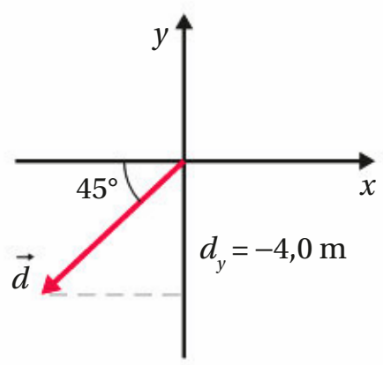
\includegraphics[scale=0.35]{vettored.png}   \end{center} \end{figure}\\\
\begin{oneparchoices}
  \choice 5,7 m; 4,0 m
  \choice -5,7 m; 4,0 m
  \choice 5,7 m; -4,0 m
  \choice -5,7 m; -4,0 m
\end{oneparchoices}

    
\question Come si chiama il satellite naturale della Terra?\\\
\begin{oneparchoices}
  \choice Sole
  \choice ISS
  \choice Luna
  \choice Marte
\end{oneparchoices}

    
\question Seguendo la mappa di un tesoro, un pirata cammina per 2,00~km verso nord-est, poi per 5,00~km verso est, quindi per 2,00~km verso sud-est e infine per 3,00~km verso ovest. Arrivato alla fine del percorso a che distanza si trova dalla posizione che occupava alla partenza?\\\
\begin{oneparchoices}
  \choice 4,59 km
  \choice 6,32 km
  \choice 4,83 km
  \choice 4,76 km
\end{oneparchoices}

    
\question Un gatto percorre 90,0~m verso sud e poi prosegue per altri 120~m verso ovest. Lo spostamento e la distanza percorsa sono rispettivamente\\\
\begin{oneparchoices}
  \choice 150~m e 210~m
  \choice 30~m e 210~m
  \choice 210~m e 210~m
  \choice 210~m e 150~m
\end{oneparchoices}

    
\question Il modulo del vettore $\vec{A}(3;4)$ è\\\
\begin{oneparchoices}
  \choice 8
  \choice 5
  \choice 25
  \choice 12
\end{oneparchoices}

    
\question Di che colore era il cavallo bianco di Napoleone?\\\
\begin{oneparchoices}
  \choice Verde
  \choice Bianco
  \choice Marrone
  \choice Blu 
\end{oneparchoices}

    
\end{questions}

    
    \newpage
    
    

        \begin{center} 
        \fbox{\fbox{\parbox{17cm}{\centering Introduzione al quiz\\\ Modello n. 20                       
        }}}
        \end{center}
\begin{questions}

    
\question Se mischio blu e giallo che colore ottengo?\\\
\begin{oneparchoices}
  \choice Giallu
  \choice Blallo
  \choice Verde
  \choice Rosso
\end{oneparchoices}

    
\question Seguendo la mappa di un tesoro, un pirata cammina per 2,00~km verso nord-est, poi per 5,00~km verso est, quindi per 2,00~km verso sud-est e infine per 3,00~km verso ovest. Arrivato alla fine del percorso a che distanza si trova dalla posizione che occupava alla partenza?\\\
\begin{oneparchoices}
  \choice 4,76 km
  \choice 4,83 km
  \choice 4,59 km
  \choice 6,32 km
\end{oneparchoices}

    
\question Raddoppiando la distanza tra due cariche elettriche puntiformi, la forza elettrostatica diminuisce del\\\
\begin{oneparchoices}
  \choice 75\%
  \choice 25\%
  \choice 90\%
  \choice 50\%
\end{oneparchoices}

    
\question In che anno pare sia nato Gesù?\\\
\begin{oneparchoices}
  \choice 20
  \choice 2019
  \choice -80
  \choice 0
\end{oneparchoices}

    
\question Di che colore era il cavallo bianco di Napoleone?\\\
\begin{oneparchoices}
  \choice Verde
  \choice Bianco
  \choice Blu 
  \choice Marrone
\end{oneparchoices}

    
\question Come si chiama il satellite naturale della Terra?\\\
\begin{oneparchoices}
  \choice Sole
  \choice Marte
  \choice Luna
  \choice ISS
\end{oneparchoices}

    
\question Il modulo del vettore $\vec{A}(3;4)$ è\\\
\begin{oneparchoices}
  \choice 8
  \choice 25
  \choice 12
  \choice 5
\end{oneparchoices}

    
\question Qual è la capitale d’Italia?\\\
\begin{oneparchoices}
  \choice Berlino
  \choice Parigi
  \choice Roma
  \choice Milano
\end{oneparchoices}

    
\question I due vettori $\vec{a}$ e $\vec{b}$ hanno lo stesso modulo e la stessa direzione. Quale delle seguenti affermazioni è falsa?\\\
\begin{oneparchoices}
  \choice La loro somma è sicuramente nulla
  \choice La loro somma non può mai essere zero
  \choice Tutte le altre
  \choice I due vettori sono sicuramente uguali
\end{oneparchoices}

    
\question In quale anno il COVID ha fatto la sua comparsa?\\\
\begin{oneparchoices}
  \choice 2001
  \choice 1943
  \choice 2020
  \choice 2019
\end{oneparchoices}

    
\question Un gatto percorre 90,0~m verso sud e poi prosegue per altri 120~m verso ovest. Lo spostamento e la distanza percorsa sono rispettivamente\\\
\begin{oneparchoices}
  \choice 210~m e 210~m
  \choice 30~m e 210~m
  \choice 150~m e 210~m
  \choice 210~m e 150~m
\end{oneparchoices}

    
\question Dato il vettore $\vec{d}$ in figura, determina il modulo e la componente $d_x$: \begin{figure}[h!]   \begin{center}     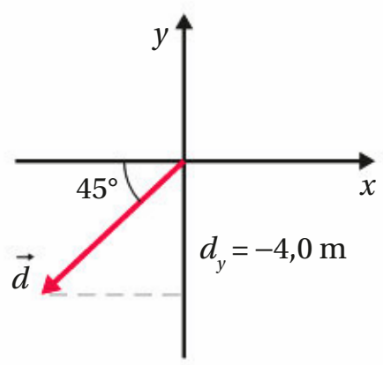
\includegraphics[scale=0.35]{vettored.png}   \end{center} \end{figure}\\\
\begin{oneparchoices}
  \choice -5,7 m; -4,0 m
  \choice 5,7 m; 4,0 m
  \choice -5,7 m; 4,0 m
  \choice 5,7 m; -4,0 m
\end{oneparchoices}

    
\end{questions}

    
    \newpage
    
    

        \begin{center} 
        \fbox{\fbox{\parbox{17cm}{\centering Introduzione al quiz\\\ Modello n. 21                       
        }}}
        \end{center}
\begin{questions}

    
\question Un gatto percorre 90,0~m verso sud e poi prosegue per altri 120~m verso ovest. Lo spostamento e la distanza percorsa sono rispettivamente\\\
\begin{oneparchoices}
  \choice 210~m e 210~m
  \choice 150~m e 210~m
  \choice 30~m e 210~m
  \choice 210~m e 150~m
\end{oneparchoices}

    
\question Il modulo del vettore $\vec{A}(3;4)$ è\\\
\begin{oneparchoices}
  \choice 25
  \choice 8
  \choice 12
  \choice 5
\end{oneparchoices}

    
\question Qual è la capitale d’Italia?\\\
\begin{oneparchoices}
  \choice Milano
  \choice Parigi
  \choice Berlino
  \choice Roma
\end{oneparchoices}

    
\question I due vettori $\vec{a}$ e $\vec{b}$ hanno lo stesso modulo e la stessa direzione. Quale delle seguenti affermazioni è falsa?\\\
\begin{oneparchoices}
  \choice La loro somma non può mai essere zero
  \choice I due vettori sono sicuramente uguali
  \choice Tutte le altre
  \choice La loro somma è sicuramente nulla
\end{oneparchoices}

    
\question Come si chiama il satellite naturale della Terra?\\\
\begin{oneparchoices}
  \choice Sole
  \choice Marte
  \choice ISS
  \choice Luna
\end{oneparchoices}

    
\question In quale anno il COVID ha fatto la sua comparsa?\\\
\begin{oneparchoices}
  \choice 2001
  \choice 2020
  \choice 1943
  \choice 2019
\end{oneparchoices}

    
\question Se mischio blu e giallo che colore ottengo?\\\
\begin{oneparchoices}
  \choice Giallu
  \choice Verde
  \choice Blallo
  \choice Rosso
\end{oneparchoices}

    
\question In che anno pare sia nato Gesù?\\\
\begin{oneparchoices}
  \choice 20
  \choice 0
  \choice 2019
  \choice -80
\end{oneparchoices}

    
\question Dato il vettore $\vec{d}$ in figura, determina il modulo e la componente $d_x$: \begin{figure}[h!]   \begin{center}     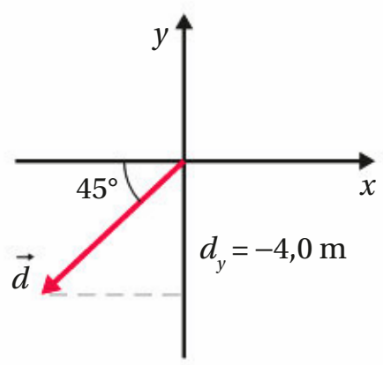
\includegraphics[scale=0.35]{vettored.png}   \end{center} \end{figure}\\\
\begin{oneparchoices}
  \choice 5,7 m; -4,0 m
  \choice -5,7 m; 4,0 m
  \choice 5,7 m; 4,0 m
  \choice -5,7 m; -4,0 m
\end{oneparchoices}

    
\question Di che colore era il cavallo bianco di Napoleone?\\\
\begin{oneparchoices}
  \choice Blu 
  \choice Verde
  \choice Marrone
  \choice Bianco
\end{oneparchoices}

    
\question Raddoppiando la distanza tra due cariche elettriche puntiformi, la forza elettrostatica diminuisce del\\\
\begin{oneparchoices}
  \choice 50\%
  \choice 75\%
  \choice 25\%
  \choice 90\%
\end{oneparchoices}

    
\question Seguendo la mappa di un tesoro, un pirata cammina per 2,00~km verso nord-est, poi per 5,00~km verso est, quindi per 2,00~km verso sud-est e infine per 3,00~km verso ovest. Arrivato alla fine del percorso a che distanza si trova dalla posizione che occupava alla partenza?\\\
\begin{oneparchoices}
  \choice 4,83 km
  \choice 4,76 km
  \choice 4,59 km
  \choice 6,32 km
\end{oneparchoices}

    
\end{questions}

    
    \newpage
    
    

        \begin{center} 
        \fbox{\fbox{\parbox{17cm}{\centering Introduzione al quiz\\\ Modello n. 22                       
        }}}
        \end{center}
\begin{questions}

    
\question Seguendo la mappa di un tesoro, un pirata cammina per 2,00~km verso nord-est, poi per 5,00~km verso est, quindi per 2,00~km verso sud-est e infine per 3,00~km verso ovest. Arrivato alla fine del percorso a che distanza si trova dalla posizione che occupava alla partenza?\\\
\begin{oneparchoices}
  \choice 4,59 km
  \choice 6,32 km
  \choice 4,76 km
  \choice 4,83 km
\end{oneparchoices}

    
\question Un gatto percorre 90,0~m verso sud e poi prosegue per altri 120~m verso ovest. Lo spostamento e la distanza percorsa sono rispettivamente\\\
\begin{oneparchoices}
  \choice 30~m e 210~m
  \choice 210~m e 210~m
  \choice 210~m e 150~m
  \choice 150~m e 210~m
\end{oneparchoices}

    
\question In quale anno il COVID ha fatto la sua comparsa?\\\
\begin{oneparchoices}
  \choice 2019
  \choice 1943
  \choice 2001
  \choice 2020
\end{oneparchoices}

    
\question In che anno pare sia nato Gesù?\\\
\begin{oneparchoices}
  \choice -80
  \choice 0
  \choice 20
  \choice 2019
\end{oneparchoices}

    
\question Dato il vettore $\vec{d}$ in figura, determina il modulo e la componente $d_x$: \begin{figure}[h!]   \begin{center}     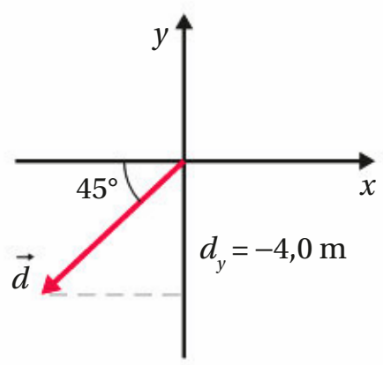
\includegraphics[scale=0.35]{vettored.png}   \end{center} \end{figure}\\\
\begin{oneparchoices}
  \choice 5,7 m; 4,0 m
  \choice -5,7 m; 4,0 m
  \choice -5,7 m; -4,0 m
  \choice 5,7 m; -4,0 m
\end{oneparchoices}

    
\question Qual è la capitale d’Italia?\\\
\begin{oneparchoices}
  \choice Milano
  \choice Roma
  \choice Parigi
  \choice Berlino
\end{oneparchoices}

    
\question Il modulo del vettore $\vec{A}(3;4)$ è\\\
\begin{oneparchoices}
  \choice 12
  \choice 5
  \choice 8
  \choice 25
\end{oneparchoices}

    
\question Come si chiama il satellite naturale della Terra?\\\
\begin{oneparchoices}
  \choice Sole
  \choice Luna
  \choice ISS
  \choice Marte
\end{oneparchoices}

    
\question I due vettori $\vec{a}$ e $\vec{b}$ hanno lo stesso modulo e la stessa direzione. Quale delle seguenti affermazioni è falsa?\\\
\begin{oneparchoices}
  \choice I due vettori sono sicuramente uguali
  \choice La loro somma non può mai essere zero
  \choice La loro somma è sicuramente nulla
  \choice Tutte le altre
\end{oneparchoices}

    
\question Se mischio blu e giallo che colore ottengo?\\\
\begin{oneparchoices}
  \choice Giallu
  \choice Rosso
  \choice Blallo
  \choice Verde
\end{oneparchoices}

    
\question Di che colore era il cavallo bianco di Napoleone?\\\
\begin{oneparchoices}
  \choice Bianco
  \choice Verde
  \choice Marrone
  \choice Blu 
\end{oneparchoices}

    
\question Raddoppiando la distanza tra due cariche elettriche puntiformi, la forza elettrostatica diminuisce del\\\
\begin{oneparchoices}
  \choice 75\%
  \choice 90\%
  \choice 50\%
  \choice 25\%
\end{oneparchoices}

    
\end{questions}

    
    \newpage
    
    

        \begin{center} 
        \fbox{\fbox{\parbox{17cm}{\centering Introduzione al quiz\\\ Modello n. 23                       
        }}}
        \end{center}
\begin{questions}

    
\question Se mischio blu e giallo che colore ottengo?\\\
\begin{oneparchoices}
  \choice Verde
  \choice Blallo
  \choice Giallu
  \choice Rosso
\end{oneparchoices}

    
\question Qual è la capitale d’Italia?\\\
\begin{oneparchoices}
  \choice Roma
  \choice Parigi
  \choice Berlino
  \choice Milano
\end{oneparchoices}

    
\question In quale anno il COVID ha fatto la sua comparsa?\\\
\begin{oneparchoices}
  \choice 1943
  \choice 2001
  \choice 2019
  \choice 2020
\end{oneparchoices}

    
\question Il modulo del vettore $\vec{A}(3;4)$ è\\\
\begin{oneparchoices}
  \choice 8
  \choice 12
  \choice 25
  \choice 5
\end{oneparchoices}

    
\question Seguendo la mappa di un tesoro, un pirata cammina per 2,00~km verso nord-est, poi per 5,00~km verso est, quindi per 2,00~km verso sud-est e infine per 3,00~km verso ovest. Arrivato alla fine del percorso a che distanza si trova dalla posizione che occupava alla partenza?\\\
\begin{oneparchoices}
  \choice 4,76 km
  \choice 4,59 km
  \choice 4,83 km
  \choice 6,32 km
\end{oneparchoices}

    
\question Raddoppiando la distanza tra due cariche elettriche puntiformi, la forza elettrostatica diminuisce del\\\
\begin{oneparchoices}
  \choice 25\%
  \choice 90\%
  \choice 50\%
  \choice 75\%
\end{oneparchoices}

    
\question I due vettori $\vec{a}$ e $\vec{b}$ hanno lo stesso modulo e la stessa direzione. Quale delle seguenti affermazioni è falsa?\\\
\begin{oneparchoices}
  \choice La loro somma è sicuramente nulla
  \choice La loro somma non può mai essere zero
  \choice Tutte le altre
  \choice I due vettori sono sicuramente uguali
\end{oneparchoices}

    
\question Dato il vettore $\vec{d}$ in figura, determina il modulo e la componente $d_x$: \begin{figure}[h!]   \begin{center}     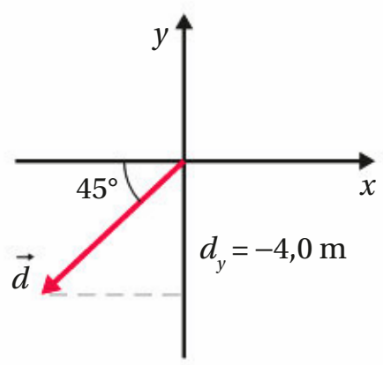
\includegraphics[scale=0.35]{vettored.png}   \end{center} \end{figure}\\\
\begin{oneparchoices}
  \choice 5,7 m; 4,0 m
  \choice -5,7 m; 4,0 m
  \choice 5,7 m; -4,0 m
  \choice -5,7 m; -4,0 m
\end{oneparchoices}

    
\question Di che colore era il cavallo bianco di Napoleone?\\\
\begin{oneparchoices}
  \choice Blu 
  \choice Verde
  \choice Bianco
  \choice Marrone
\end{oneparchoices}

    
\question In che anno pare sia nato Gesù?\\\
\begin{oneparchoices}
  \choice 0
  \choice 2019
  \choice 20
  \choice -80
\end{oneparchoices}

    
\question Un gatto percorre 90,0~m verso sud e poi prosegue per altri 120~m verso ovest. Lo spostamento e la distanza percorsa sono rispettivamente\\\
\begin{oneparchoices}
  \choice 210~m e 150~m
  \choice 30~m e 210~m
  \choice 150~m e 210~m
  \choice 210~m e 210~m
\end{oneparchoices}

    
\question Come si chiama il satellite naturale della Terra?\\\
\begin{oneparchoices}
  \choice Marte
  \choice ISS
  \choice Sole
  \choice Luna
\end{oneparchoices}

    
\end{questions}

    
    \newpage
    
    

        \begin{center} 
        \fbox{\fbox{\parbox{17cm}{\centering Introduzione al quiz\\\ Modello n. 24                       
        }}}
        \end{center}
\begin{questions}

    
\question Di che colore era il cavallo bianco di Napoleone?\\\
\begin{oneparchoices}
  \choice Verde
  \choice Bianco
  \choice Blu 
  \choice Marrone
\end{oneparchoices}

    
\question In quale anno il COVID ha fatto la sua comparsa?\\\
\begin{oneparchoices}
  \choice 2019
  \choice 1943
  \choice 2001
  \choice 2020
\end{oneparchoices}

    
\question In che anno pare sia nato Gesù?\\\
\begin{oneparchoices}
  \choice 0
  \choice 2019
  \choice 20
  \choice -80
\end{oneparchoices}

    
\question Seguendo la mappa di un tesoro, un pirata cammina per 2,00~km verso nord-est, poi per 5,00~km verso est, quindi per 2,00~km verso sud-est e infine per 3,00~km verso ovest. Arrivato alla fine del percorso a che distanza si trova dalla posizione che occupava alla partenza?\\\
\begin{oneparchoices}
  \choice 4,59 km
  \choice 6,32 km
  \choice 4,83 km
  \choice 4,76 km
\end{oneparchoices}

    
\question Qual è la capitale d’Italia?\\\
\begin{oneparchoices}
  \choice Parigi
  \choice Berlino
  \choice Roma
  \choice Milano
\end{oneparchoices}

    
\question Come si chiama il satellite naturale della Terra?\\\
\begin{oneparchoices}
  \choice Marte
  \choice Luna
  \choice Sole
  \choice ISS
\end{oneparchoices}

    
\question I due vettori $\vec{a}$ e $\vec{b}$ hanno lo stesso modulo e la stessa direzione. Quale delle seguenti affermazioni è falsa?\\\
\begin{oneparchoices}
  \choice La loro somma è sicuramente nulla
  \choice La loro somma non può mai essere zero
  \choice I due vettori sono sicuramente uguali
  \choice Tutte le altre
\end{oneparchoices}

    
\question Se mischio blu e giallo che colore ottengo?\\\
\begin{oneparchoices}
  \choice Giallu
  \choice Blallo
  \choice Rosso
  \choice Verde
\end{oneparchoices}

    
\question Raddoppiando la distanza tra due cariche elettriche puntiformi, la forza elettrostatica diminuisce del\\\
\begin{oneparchoices}
  \choice 25\%
  \choice 50\%
  \choice 90\%
  \choice 75\%
\end{oneparchoices}

    
\question Dato il vettore $\vec{d}$ in figura, determina il modulo e la componente $d_x$: \begin{figure}[h!]   \begin{center}     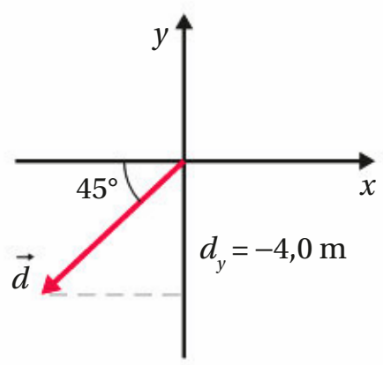
\includegraphics[scale=0.35]{vettored.png}   \end{center} \end{figure}\\\
\begin{oneparchoices}
  \choice -5,7 m; 4,0 m
  \choice 5,7 m; -4,0 m
  \choice -5,7 m; -4,0 m
  \choice 5,7 m; 4,0 m
\end{oneparchoices}

    
\question Un gatto percorre 90,0~m verso sud e poi prosegue per altri 120~m verso ovest. Lo spostamento e la distanza percorsa sono rispettivamente\\\
\begin{oneparchoices}
  \choice 210~m e 210~m
  \choice 210~m e 150~m
  \choice 150~m e 210~m
  \choice 30~m e 210~m
\end{oneparchoices}

    
\question Il modulo del vettore $\vec{A}(3;4)$ è\\\
\begin{oneparchoices}
  \choice 8
  \choice 25
  \choice 5
  \choice 12
\end{oneparchoices}

    
\end{questions}

    
    \newpage
    
    

        \begin{center} 
        \fbox{\fbox{\parbox{17cm}{\centering Introduzione al quiz\\\ Modello n. 25                       
        }}}
        \end{center}
\begin{questions}

    
\question In che anno pare sia nato Gesù?\\\
\begin{oneparchoices}
  \choice 0
  \choice -80
  \choice 2019
  \choice 20
\end{oneparchoices}

    
\question Un gatto percorre 90,0~m verso sud e poi prosegue per altri 120~m verso ovest. Lo spostamento e la distanza percorsa sono rispettivamente\\\
\begin{oneparchoices}
  \choice 30~m e 210~m
  \choice 210~m e 150~m
  \choice 150~m e 210~m
  \choice 210~m e 210~m
\end{oneparchoices}

    
\question Di che colore era il cavallo bianco di Napoleone?\\\
\begin{oneparchoices}
  \choice Blu 
  \choice Bianco
  \choice Marrone
  \choice Verde
\end{oneparchoices}

    
\question Se mischio blu e giallo che colore ottengo?\\\
\begin{oneparchoices}
  \choice Blallo
  \choice Rosso
  \choice Verde
  \choice Giallu
\end{oneparchoices}

    
\question Qual è la capitale d’Italia?\\\
\begin{oneparchoices}
  \choice Milano
  \choice Parigi
  \choice Roma
  \choice Berlino
\end{oneparchoices}

    
\question Il modulo del vettore $\vec{A}(3;4)$ è\\\
\begin{oneparchoices}
  \choice 12
  \choice 8
  \choice 25
  \choice 5
\end{oneparchoices}

    
\question Seguendo la mappa di un tesoro, un pirata cammina per 2,00~km verso nord-est, poi per 5,00~km verso est, quindi per 2,00~km verso sud-est e infine per 3,00~km verso ovest. Arrivato alla fine del percorso a che distanza si trova dalla posizione che occupava alla partenza?\\\
\begin{oneparchoices}
  \choice 6,32 km
  \choice 4,59 km
  \choice 4,83 km
  \choice 4,76 km
\end{oneparchoices}

    
\question Come si chiama il satellite naturale della Terra?\\\
\begin{oneparchoices}
  \choice Sole
  \choice ISS
  \choice Marte
  \choice Luna
\end{oneparchoices}

    
\question Dato il vettore $\vec{d}$ in figura, determina il modulo e la componente $d_x$: \begin{figure}[h!]   \begin{center}     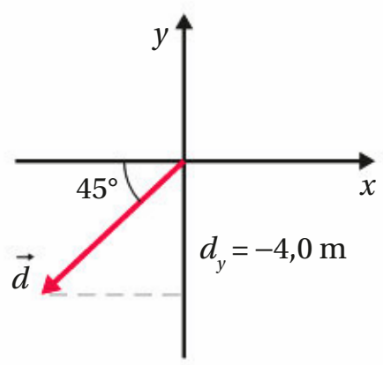
\includegraphics[scale=0.35]{vettored.png}   \end{center} \end{figure}\\\
\begin{oneparchoices}
  \choice -5,7 m; -4,0 m
  \choice -5,7 m; 4,0 m
  \choice 5,7 m; -4,0 m
  \choice 5,7 m; 4,0 m
\end{oneparchoices}

    
\question Raddoppiando la distanza tra due cariche elettriche puntiformi, la forza elettrostatica diminuisce del\\\
\begin{oneparchoices}
  \choice 90\%
  \choice 50\%
  \choice 75\%
  \choice 25\%
\end{oneparchoices}

    
\question In quale anno il COVID ha fatto la sua comparsa?\\\
\begin{oneparchoices}
  \choice 2019
  \choice 2001
  \choice 2020
  \choice 1943
\end{oneparchoices}

    
\question I due vettori $\vec{a}$ e $\vec{b}$ hanno lo stesso modulo e la stessa direzione. Quale delle seguenti affermazioni è falsa?\\\
\begin{oneparchoices}
  \choice Tutte le altre
  \choice I due vettori sono sicuramente uguali
  \choice La loro somma non può mai essere zero
  \choice La loro somma è sicuramente nulla
\end{oneparchoices}

    
\end{questions}

    
    \newpage
    
    

        \begin{center} 
        \fbox{\fbox{\parbox{17cm}{\centering Introduzione al quiz\\\ Modello n. 26                       
        }}}
        \end{center}
\begin{questions}

    
\question Qual è la capitale d’Italia?\\\
\begin{oneparchoices}
  \choice Milano
  \choice Parigi
  \choice Berlino
  \choice Roma
\end{oneparchoices}

    
\question Di che colore era il cavallo bianco di Napoleone?\\\
\begin{oneparchoices}
  \choice Marrone
  \choice Verde
  \choice Blu 
  \choice Bianco
\end{oneparchoices}

    
\question Seguendo la mappa di un tesoro, un pirata cammina per 2,00~km verso nord-est, poi per 5,00~km verso est, quindi per 2,00~km verso sud-est e infine per 3,00~km verso ovest. Arrivato alla fine del percorso a che distanza si trova dalla posizione che occupava alla partenza?\\\
\begin{oneparchoices}
  \choice 4,59 km
  \choice 4,76 km
  \choice 6,32 km
  \choice 4,83 km
\end{oneparchoices}

    
\question Come si chiama il satellite naturale della Terra?\\\
\begin{oneparchoices}
  \choice Sole
  \choice Marte
  \choice ISS
  \choice Luna
\end{oneparchoices}

    
\question Se mischio blu e giallo che colore ottengo?\\\
\begin{oneparchoices}
  \choice Rosso
  \choice Giallu
  \choice Verde
  \choice Blallo
\end{oneparchoices}

    
\question I due vettori $\vec{a}$ e $\vec{b}$ hanno lo stesso modulo e la stessa direzione. Quale delle seguenti affermazioni è falsa?\\\
\begin{oneparchoices}
  \choice Tutte le altre
  \choice La loro somma non può mai essere zero
  \choice La loro somma è sicuramente nulla
  \choice I due vettori sono sicuramente uguali
\end{oneparchoices}

    
\question In che anno pare sia nato Gesù?\\\
\begin{oneparchoices}
  \choice 0
  \choice 20
  \choice -80
  \choice 2019
\end{oneparchoices}

    
\question Dato il vettore $\vec{d}$ in figura, determina il modulo e la componente $d_x$: \begin{figure}[h!]   \begin{center}     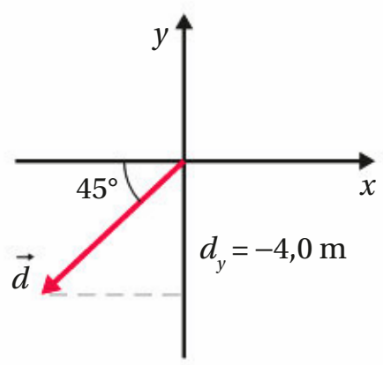
\includegraphics[scale=0.35]{vettored.png}   \end{center} \end{figure}\\\
\begin{oneparchoices}
  \choice 5,7 m; -4,0 m
  \choice -5,7 m; -4,0 m
  \choice 5,7 m; 4,0 m
  \choice -5,7 m; 4,0 m
\end{oneparchoices}

    
\question Raddoppiando la distanza tra due cariche elettriche puntiformi, la forza elettrostatica diminuisce del\\\
\begin{oneparchoices}
  \choice 50\%
  \choice 25\%
  \choice 75\%
  \choice 90\%
\end{oneparchoices}

    
\question Un gatto percorre 90,0~m verso sud e poi prosegue per altri 120~m verso ovest. Lo spostamento e la distanza percorsa sono rispettivamente\\\
\begin{oneparchoices}
  \choice 210~m e 210~m
  \choice 30~m e 210~m
  \choice 150~m e 210~m
  \choice 210~m e 150~m
\end{oneparchoices}

    
\question In quale anno il COVID ha fatto la sua comparsa?\\\
\begin{oneparchoices}
  \choice 1943
  \choice 2020
  \choice 2019
  \choice 2001
\end{oneparchoices}

    
\question Il modulo del vettore $\vec{A}(3;4)$ è\\\
\begin{oneparchoices}
  \choice 25
  \choice 5
  \choice 12
  \choice 8
\end{oneparchoices}

    
\end{questions}

    
    \newpage
    
    

        \begin{center} 
        \fbox{\fbox{\parbox{17cm}{\centering Introduzione al quiz\\\ Modello n. 27                       
        }}}
        \end{center}
\begin{questions}

    
\question Se mischio blu e giallo che colore ottengo?\\\
\begin{oneparchoices}
  \choice Rosso
  \choice Giallu
  \choice Blallo
  \choice Verde
\end{oneparchoices}

    
\question Come si chiama il satellite naturale della Terra?\\\
\begin{oneparchoices}
  \choice Luna
  \choice Sole
  \choice ISS
  \choice Marte
\end{oneparchoices}

    
\question Raddoppiando la distanza tra due cariche elettriche puntiformi, la forza elettrostatica diminuisce del\\\
\begin{oneparchoices}
  \choice 75\%
  \choice 25\%
  \choice 50\%
  \choice 90\%
\end{oneparchoices}

    
\question I due vettori $\vec{a}$ e $\vec{b}$ hanno lo stesso modulo e la stessa direzione. Quale delle seguenti affermazioni è falsa?\\\
\begin{oneparchoices}
  \choice I due vettori sono sicuramente uguali
  \choice La loro somma è sicuramente nulla
  \choice La loro somma non può mai essere zero
  \choice Tutte le altre
\end{oneparchoices}

    
\question In che anno pare sia nato Gesù?\\\
\begin{oneparchoices}
  \choice 0
  \choice 20
  \choice 2019
  \choice -80
\end{oneparchoices}

    
\question Seguendo la mappa di un tesoro, un pirata cammina per 2,00~km verso nord-est, poi per 5,00~km verso est, quindi per 2,00~km verso sud-est e infine per 3,00~km verso ovest. Arrivato alla fine del percorso a che distanza si trova dalla posizione che occupava alla partenza?\\\
\begin{oneparchoices}
  \choice 6,32 km
  \choice 4,76 km
  \choice 4,59 km
  \choice 4,83 km
\end{oneparchoices}

    
\question Dato il vettore $\vec{d}$ in figura, determina il modulo e la componente $d_x$: \begin{figure}[h!]   \begin{center}     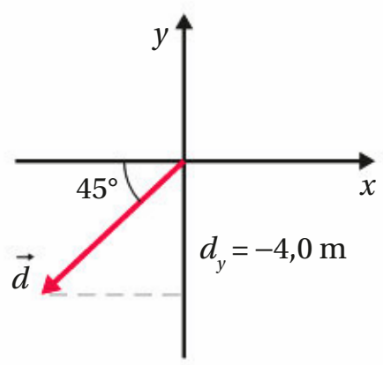
\includegraphics[scale=0.35]{vettored.png}   \end{center} \end{figure}\\\
\begin{oneparchoices}
  \choice -5,7 m; 4,0 m
  \choice -5,7 m; -4,0 m
  \choice 5,7 m; 4,0 m
  \choice 5,7 m; -4,0 m
\end{oneparchoices}

    
\question Un gatto percorre 90,0~m verso sud e poi prosegue per altri 120~m verso ovest. Lo spostamento e la distanza percorsa sono rispettivamente\\\
\begin{oneparchoices}
  \choice 210~m e 210~m
  \choice 150~m e 210~m
  \choice 30~m e 210~m
  \choice 210~m e 150~m
\end{oneparchoices}

    
\question Il modulo del vettore $\vec{A}(3;4)$ è\\\
\begin{oneparchoices}
  \choice 25
  \choice 12
  \choice 8
  \choice 5
\end{oneparchoices}

    
\question Qual è la capitale d’Italia?\\\
\begin{oneparchoices}
  \choice Berlino
  \choice Milano
  \choice Parigi
  \choice Roma
\end{oneparchoices}

    
\question Di che colore era il cavallo bianco di Napoleone?\\\
\begin{oneparchoices}
  \choice Verde
  \choice Marrone
  \choice Blu 
  \choice Bianco
\end{oneparchoices}

    
\question In quale anno il COVID ha fatto la sua comparsa?\\\
\begin{oneparchoices}
  \choice 2020
  \choice 2001
  \choice 1943
  \choice 2019
\end{oneparchoices}

    
\end{questions}

    
    \newpage
    
    

        \begin{center} 
        \fbox{\fbox{\parbox{17cm}{\centering Introduzione al quiz\\\ Modello n. 28                       
        }}}
        \end{center}
\begin{questions}

    
\question Se mischio blu e giallo che colore ottengo?\\\
\begin{oneparchoices}
  \choice Giallu
  \choice Rosso
  \choice Blallo
  \choice Verde
\end{oneparchoices}

    
\question In quale anno il COVID ha fatto la sua comparsa?\\\
\begin{oneparchoices}
  \choice 1943
  \choice 2020
  \choice 2019
  \choice 2001
\end{oneparchoices}

    
\question Seguendo la mappa di un tesoro, un pirata cammina per 2,00~km verso nord-est, poi per 5,00~km verso est, quindi per 2,00~km verso sud-est e infine per 3,00~km verso ovest. Arrivato alla fine del percorso a che distanza si trova dalla posizione che occupava alla partenza?\\\
\begin{oneparchoices}
  \choice 4,59 km
  \choice 4,76 km
  \choice 4,83 km
  \choice 6,32 km
\end{oneparchoices}

    
\question Come si chiama il satellite naturale della Terra?\\\
\begin{oneparchoices}
  \choice Sole
  \choice ISS
  \choice Marte
  \choice Luna
\end{oneparchoices}

    
\question In che anno pare sia nato Gesù?\\\
\begin{oneparchoices}
  \choice 20
  \choice 0
  \choice 2019
  \choice -80
\end{oneparchoices}

    
\question Raddoppiando la distanza tra due cariche elettriche puntiformi, la forza elettrostatica diminuisce del\\\
\begin{oneparchoices}
  \choice 50\%
  \choice 90\%
  \choice 75\%
  \choice 25\%
\end{oneparchoices}

    
\question I due vettori $\vec{a}$ e $\vec{b}$ hanno lo stesso modulo e la stessa direzione. Quale delle seguenti affermazioni è falsa?\\\
\begin{oneparchoices}
  \choice La loro somma è sicuramente nulla
  \choice I due vettori sono sicuramente uguali
  \choice Tutte le altre
  \choice La loro somma non può mai essere zero
\end{oneparchoices}

    
\question Un gatto percorre 90,0~m verso sud e poi prosegue per altri 120~m verso ovest. Lo spostamento e la distanza percorsa sono rispettivamente\\\
\begin{oneparchoices}
  \choice 30~m e 210~m
  \choice 150~m e 210~m
  \choice 210~m e 210~m
  \choice 210~m e 150~m
\end{oneparchoices}

    
\question Di che colore era il cavallo bianco di Napoleone?\\\
\begin{oneparchoices}
  \choice Verde
  \choice Bianco
  \choice Blu 
  \choice Marrone
\end{oneparchoices}

    
\question Il modulo del vettore $\vec{A}(3;4)$ è\\\
\begin{oneparchoices}
  \choice 25
  \choice 8
  \choice 12
  \choice 5
\end{oneparchoices}

    
\question Dato il vettore $\vec{d}$ in figura, determina il modulo e la componente $d_x$: \begin{figure}[h!]   \begin{center}     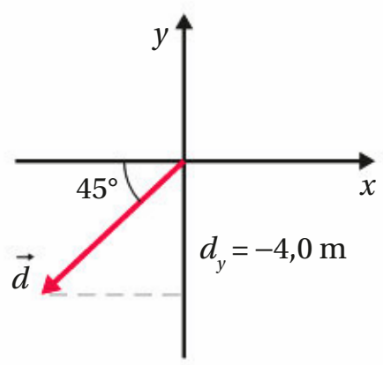
\includegraphics[scale=0.35]{vettored.png}   \end{center} \end{figure}\\\
\begin{oneparchoices}
  \choice 5,7 m; -4,0 m
  \choice -5,7 m; -4,0 m
  \choice 5,7 m; 4,0 m
  \choice -5,7 m; 4,0 m
\end{oneparchoices}

    
\question Qual è la capitale d’Italia?\\\
\begin{oneparchoices}
  \choice Roma
  \choice Parigi
  \choice Milano
  \choice Berlino
\end{oneparchoices}

    
\end{questions}

    
    \newpage
    
    

        \begin{center} 
        \fbox{\fbox{\parbox{17cm}{\centering Introduzione al quiz\\\ Modello n. 29                       
        }}}
        \end{center}
\begin{questions}

    
\question Il modulo del vettore $\vec{A}(3;4)$ è\\\
\begin{oneparchoices}
  \choice 8
  \choice 5
  \choice 25
  \choice 12
\end{oneparchoices}

    
\question Un gatto percorre 90,0~m verso sud e poi prosegue per altri 120~m verso ovest. Lo spostamento e la distanza percorsa sono rispettivamente\\\
\begin{oneparchoices}
  \choice 210~m e 210~m
  \choice 30~m e 210~m
  \choice 150~m e 210~m
  \choice 210~m e 150~m
\end{oneparchoices}

    
\question Come si chiama il satellite naturale della Terra?\\\
\begin{oneparchoices}
  \choice Luna
  \choice ISS
  \choice Sole
  \choice Marte
\end{oneparchoices}

    
\question Seguendo la mappa di un tesoro, un pirata cammina per 2,00~km verso nord-est, poi per 5,00~km verso est, quindi per 2,00~km verso sud-est e infine per 3,00~km verso ovest. Arrivato alla fine del percorso a che distanza si trova dalla posizione che occupava alla partenza?\\\
\begin{oneparchoices}
  \choice 6,32 km
  \choice 4,76 km
  \choice 4,83 km
  \choice 4,59 km
\end{oneparchoices}

    
\question I due vettori $\vec{a}$ e $\vec{b}$ hanno lo stesso modulo e la stessa direzione. Quale delle seguenti affermazioni è falsa?\\\
\begin{oneparchoices}
  \choice La loro somma non può mai essere zero
  \choice Tutte le altre
  \choice La loro somma è sicuramente nulla
  \choice I due vettori sono sicuramente uguali
\end{oneparchoices}

    
\question Dato il vettore $\vec{d}$ in figura, determina il modulo e la componente $d_x$: \begin{figure}[h!]   \begin{center}     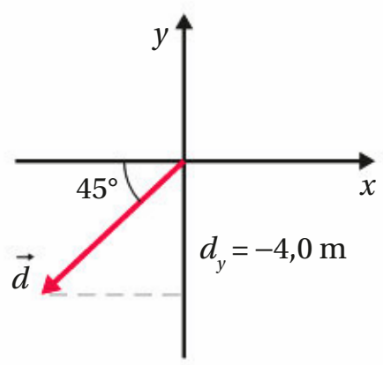
\includegraphics[scale=0.35]{vettored.png}   \end{center} \end{figure}\\\
\begin{oneparchoices}
  \choice -5,7 m; -4,0 m
  \choice -5,7 m; 4,0 m
  \choice 5,7 m; 4,0 m
  \choice 5,7 m; -4,0 m
\end{oneparchoices}

    
\question Qual è la capitale d’Italia?\\\
\begin{oneparchoices}
  \choice Roma
  \choice Parigi
  \choice Berlino
  \choice Milano
\end{oneparchoices}

    
\question In che anno pare sia nato Gesù?\\\
\begin{oneparchoices}
  \choice 2019
  \choice -80
  \choice 0
  \choice 20
\end{oneparchoices}

    
\question In quale anno il COVID ha fatto la sua comparsa?\\\
\begin{oneparchoices}
  \choice 2001
  \choice 2020
  \choice 1943
  \choice 2019
\end{oneparchoices}

    
\question Di che colore era il cavallo bianco di Napoleone?\\\
\begin{oneparchoices}
  \choice Blu 
  \choice Bianco
  \choice Verde
  \choice Marrone
\end{oneparchoices}

    
\question Raddoppiando la distanza tra due cariche elettriche puntiformi, la forza elettrostatica diminuisce del\\\
\begin{oneparchoices}
  \choice 75\%
  \choice 90\%
  \choice 50\%
  \choice 25\%
\end{oneparchoices}

    
\question Se mischio blu e giallo che colore ottengo?\\\
\begin{oneparchoices}
  \choice Giallu
  \choice Verde
  \choice Blallo
  \choice Rosso
\end{oneparchoices}

    
\end{questions}

    
    \newpage
    
    

        \begin{center} 
        \fbox{\fbox{\parbox{17cm}{\centering Introduzione al quiz\\\ Modello n. 30                       
        }}}
        \end{center}
\begin{questions}

    
\question In quale anno il COVID ha fatto la sua comparsa?\\\
\begin{oneparchoices}
  \choice 2019
  \choice 1943
  \choice 2001
  \choice 2020
\end{oneparchoices}

    
\question Seguendo la mappa di un tesoro, un pirata cammina per 2,00~km verso nord-est, poi per 5,00~km verso est, quindi per 2,00~km verso sud-est e infine per 3,00~km verso ovest. Arrivato alla fine del percorso a che distanza si trova dalla posizione che occupava alla partenza?\\\
\begin{oneparchoices}
  \choice 6,32 km
  \choice 4,76 km
  \choice 4,59 km
  \choice 4,83 km
\end{oneparchoices}

    
\question In che anno pare sia nato Gesù?\\\
\begin{oneparchoices}
  \choice 0
  \choice -80
  \choice 20
  \choice 2019
\end{oneparchoices}

    
\question Il modulo del vettore $\vec{A}(3;4)$ è\\\
\begin{oneparchoices}
  \choice 25
  \choice 8
  \choice 5
  \choice 12
\end{oneparchoices}

    
\question Un gatto percorre 90,0~m verso sud e poi prosegue per altri 120~m verso ovest. Lo spostamento e la distanza percorsa sono rispettivamente\\\
\begin{oneparchoices}
  \choice 150~m e 210~m
  \choice 210~m e 150~m
  \choice 30~m e 210~m
  \choice 210~m e 210~m
\end{oneparchoices}

    
\question Dato il vettore $\vec{d}$ in figura, determina il modulo e la componente $d_x$: \begin{figure}[h!]   \begin{center}     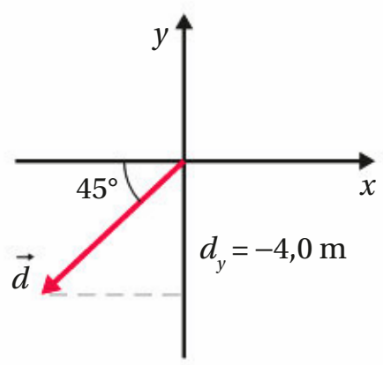
\includegraphics[scale=0.35]{vettored.png}   \end{center} \end{figure}\\\
\begin{oneparchoices}
  \choice -5,7 m; 4,0 m
  \choice 5,7 m; 4,0 m
  \choice 5,7 m; -4,0 m
  \choice -5,7 m; -4,0 m
\end{oneparchoices}

    
\question Come si chiama il satellite naturale della Terra?\\\
\begin{oneparchoices}
  \choice Marte
  \choice Luna
  \choice Sole
  \choice ISS
\end{oneparchoices}

    
\question I due vettori $\vec{a}$ e $\vec{b}$ hanno lo stesso modulo e la stessa direzione. Quale delle seguenti affermazioni è falsa?\\\
\begin{oneparchoices}
  \choice La loro somma è sicuramente nulla
  \choice La loro somma non può mai essere zero
  \choice Tutte le altre
  \choice I due vettori sono sicuramente uguali
\end{oneparchoices}

    
\question Raddoppiando la distanza tra due cariche elettriche puntiformi, la forza elettrostatica diminuisce del\\\
\begin{oneparchoices}
  \choice 50\%
  \choice 90\%
  \choice 75\%
  \choice 25\%
\end{oneparchoices}

    
\question Se mischio blu e giallo che colore ottengo?\\\
\begin{oneparchoices}
  \choice Blallo
  \choice Verde
  \choice Rosso
  \choice Giallu
\end{oneparchoices}

    
\question Qual è la capitale d’Italia?\\\
\begin{oneparchoices}
  \choice Roma
  \choice Berlino
  \choice Milano
  \choice Parigi
\end{oneparchoices}

    
\question Di che colore era il cavallo bianco di Napoleone?\\\
\begin{oneparchoices}
  \choice Verde
  \choice Marrone
  \choice Bianco
  \choice Blu 
\end{oneparchoices}

    
\end{questions}

    
    \newpage
    
    
\end{document}
    